% Canonical HVK supplementary manuscript. The main framework narrative belongs
% in paper_hvk.tex; detailed ablations, audits, and validation live here.
\documentclass[11pt]{article}
\usepackage[margin=1in]{geometry}
\usepackage{amsmath,amsfonts,amssymb,graphicx,booktabs,cite,bm}
\usepackage[hidelinks,hypertexnames=false]{hyperref}
\usepackage{float}

\title{Supplementary Material for the Hamiltonian Vision Kernel:\\ Resource-Matched Ablations, Validation, and Reproducibility}
\author{Sparsho~Chakraborty and Dr.~Siddhartha~Patra}
\date{}

\begin{document}
\maketitle

\begin{abstract}
This supplementary material accompanies the main manuscript, \textit{Hamiltonian Vision Kernel: Symmetry-Pooled Quantum Correlator Features with Hardware Validation}. The main paper introduces HVK as a new hybrid quantum--classical architecture and establishes a feature-level, numerically verified $D_4$-equivariance construction, a scoped nonlocal representational capability, and real IBM Quantum hardware execution. Here we strengthen that framework through resource-matched multi-seed controls, held-out evaluation, leakage auditing, and complete hardware methodology. On ordinary held-out reconstruction, simple local/raw feature maps match or exceed the tested HVK feature map under the same fitted readout, a direction that also holds when a single HVK2D model is trained end-to-end by gradient descent across 150 images and evaluated on 50 held-out images never seen during training. The entangling observable channel separates only on the restricted task constructed to require nonlocal correlations, while $D_4$ pooling supplies a distinct feature-level symmetry guarantee rather than a demonstrated reconstruction advantage. We also document why an earlier multi-seed Monalisa freeze table could not be reproduced from retained artifacts, and report its replacement: a fresh, matched-budget rerun of the same nine-variant comparison, which reaches the same conclusion as the held-out result above. The available training-dynamics traces remain excluded pending a reproducible rerun. This task-dependent result sharpens HVK's design scope without changing its architectural contribution.
\end{abstract}

\tableofcontents

\section{Introduction}
The main paper presents the Hamiltonian Vision Kernel (HVK1D/HVK2D) --- a physics-informed hybrid quantum--classical image autoencoder combining matrix-product-state (MPS) patch features, a variational quantum circuit (VQC) producing a Pauli-correlator latent space, a learnable graph-Hamiltonian energy diagnostic, 2D Fourier positional encoding, and a classical decoder --- and its positive, independently verified properties. A complete account of any hybrid architecture should also ask whether its proposed representation improves performance under held-out, resource-matched controls. This document answers that question with a leakage-audited multi-seed validation suite and records provenance limitations where an earlier exploratory result cannot be reproduced from retained artifacts. The result is a rigorous complement: it defines precisely the tested boundary of the main paper's positive entanglement and $D_4$-symmetry findings and provides the evidence base for the dequantization context discussed there.

\section{Method}

\subsection{Ablation and Control Design}
The codebase implements targeted freezes and replacements for component-isolation experiments. \emph{Freeze-classical} trains only the circuit and Hamiltonian couplings while fixing the decoder and projection layers; \emph{freeze-quantum} does the reverse. \emph{No-entanglement} removes the CNOT rings, and \emph{no-energy-loss} removes the Hamiltonian regularizer. \emph{Classical-replacement} and \emph{classical-matched} replace the VQC with a tanh map; the matched version is rank-limited to the circuit's parameter count. Every retained classical control in the held-out CIFAR-10 layer is resource-matched: identical feature width (32-D) and linear-readout parameter count (2112), so residual gaps reflect feature structure rather than decoder capacity (Table~\ref{tab:resource_capacity}). Section~\ref{sec:component_provenance} distinguishes these implemented controls from the earlier Monalisa aggregate that lacks reproducible per-seed artifacts.

\subsection{Statistical Protocol}
The retained quantitative comparisons state their own replication unit and optimization budget. Capacity sweeps in Table~\ref{tab:capacity_ablation} are single-seed directional diagnostics. The held-out CIFAR-10 validation layer and the restricted pair-correlation diagnostic are multi-seed: five random seeds for the restricted diagnostic, and five random image splits (20 held-out reconstructions total) for real CIFAR-10, each using a shared linear readout trained on a disjoint image subset. For held-out reconstruction inference, paired image differences are averaged within each split seed before bootstrap and Wilcoxon calculations, so predictions sharing one fitted readout are not treated as independent replicates. Section~\ref{sec:component_provenance} explains why an earlier five-seed Monalisa freeze-isolation table is not retained as quantitative evidence.

\subsection{Leakage Auditing}
Because several of our diagnostics are deliberately constructed so that a target depends on features only some models receive, we audit every such diagnostic for a specific failure mode: a regression target that is a (near-)linear function of a quantity handed verbatim to only one candidate model, which produces an apparent representational advantage that is actually copying rather than learning. Concretely, for a target $y$ and a candidate feature block $x$, we check whether a linear or near-linear map from $x$ to $y$ achieves near-zero residual on features the target-construction code itself used to build $y$ --- if so, the feature block and the target share provenance and the diagnostic is circular regardless of model architecture. Every constructed diagnostic retained as quantitative evidence has passed this check; no retained quantitative claim depends on a diagnostic that failed it.

\subsection{Datasets and Metrics}
We use three settings, in increasing order of evidentiary weight for a generalization claim. \textit{Single-image} (\textit{Monalisa}, $256\times256$, 16 patches of $64\times64$) tests per-image optimization only. \textit{CIFAR-10 same-set} (five native $32\times32$ images) is a same-set reconstruction fit, useful for capacity/positioning comparisons but not a generalization test --- the MLP baseline's same-set PSNR exceeds $100$~dB in the best case, a memorization red flag rather than evidence of representation quality. \textit{Held-out CIFAR-10} (five random splits, disjoint train/held-out images, 20 total held-out reconstructions) and a six-dataset multi-dataset suite use CIFAR-10 \cite{Krizhevsky2009}, MNIST \cite{LeCun1998}, Fashion-MNIST \cite{Xiao2017}, and PathMNIST, BloodMNIST, and PneumoniaMNIST from MedMNIST v2 \cite{Yang2023}, plus the Wisconsin Diagnostic Breast Cancer dataset \cite{Wolberg1993} as a tabular cross-domain check. These are the settings that test a \emph{learned representation} rather than per-image memorization, and are therefore the basis for this document's central ablation claim. All settings report MSE and PSNR $=20\log_{10}(1/\sqrt{\mathrm{MSE}})$; image settings additionally report SSIM.

\section{Results}
\label{sec:results}

\subsection{Component-Ablation Provenance Audit}
\label{sec:component_provenance}
\begin{sloppypar}
An earlier draft presented a nine-variant, five-seed Monalisa freeze-isolation table. The repository does not contain the per-seed records or a machine-readable summary that reproduces those reported means and standard deviations. The retained legacy directory contains only three evaluation-control records, while \path{main2/newHVK/results/full_ablation_suite/full_ablation_summary.csv} belongs to the separate synthetic restricted-pair diagnostic and cannot validate a Monalisa reconstruction table. We therefore exclude the earlier table, its summary figure, and all quantitative attribution claims derived from it. The freeze and replacement implementations remain available for a fresh matched-budget rerun, but no decoder-necessity conclusion is drawn from the incomplete legacy artifacts. The retained evidence below instead asks the reproducible held-out question: under an identical fitted readout, do the tested HVK features outperform resource-matched classical or ablated feature maps?
\end{sloppypar}

\subsection{A Fresh, Matched-Budget Rerun of the Nine-Variant Table}
\label{sec:core_multiseed_rerun}
The fresh matched-budget rerun anticipated above is now complete. All nine variants (baseline, freeze-quantum, freeze-classical, no-entanglement, no-MPS, no-energy-loss, classical-replacement, classical-matched, random-VQC) were trained on \textit{Monalisa} at a matched 240-step budget (identical learning rate and schedule across variants), for 3 seeds each --- reduced from an initially planned 5 seeds for compute-budget reasons on this CPU-only machine (real per-patch VQC circuit cost, not a resource shortfall specific to any one variant; documented explicitly as \texttt{scope\_reduced: true} in the run's own summary file). Table~\ref{tab:core_multiseed_240} reports mean $\pm$ std PSNR and SSIM per variant, and Table~\ref{tab:core_multiseed_240_stats} gives the quantum-vs-classical/random-control comparisons, marking any gap smaller than one pooled standard deviation as not significant, following this document's established statistical-protocol convention.

\begin{table}[H]
\centering
\caption{Matched-budget (240-step) core ablation, \textit{Monalisa}, 3 seeds/variant. Freeze-classical's collapse is expected (decoder frozen, cannot learn to reconstruct) and serves as a sanity check on the ablation harness itself.}
\label{tab:core_multiseed_240}
\scriptsize
\begin{tabular}{lcc}
\toprule
Variant & PSNR (dB) & SSIM \\
\midrule
Baseline (quantum) & $33.42\pm0.02$ & $0.99385\pm0.00003$ \\
Freeze-quantum & $33.39\pm0.06$ & $0.99381\pm0.00006$ \\
No-entanglement & $33.48\pm0.02$ & $0.99392\pm0.00003$ \\
No-MPS & $33.34\pm0.05$ & $0.99374\pm0.00008$ \\
No-energy-loss & $33.44\pm0.01$ & $0.99387\pm0.00001$ \\
Classical-replacement & $33.50\pm0.01$ & $0.99395\pm0.00002$ \\
Classical-matched & $33.22\pm0.19$ & $0.99356\pm0.00027$ \\
Random-VQC & $28.09\pm0.23$ & $0.97907\pm0.00135$ \\
Freeze-classical & $10.94\pm0.00$ & $0.0219\pm0.0001$ \\
\bottomrule
\end{tabular}
\end{table}

\begin{table}[H]
\centering
\caption{Quantum-baseline-vs-control comparisons for Table~\ref{tab:core_multiseed_240}. Significance rule: gap $\geq$ pooled std of the two variants' seed-level PSNR $\Rightarrow$ significant, following this document's convention of not claiming within-noise gaps.}
\label{tab:core_multiseed_240_stats}
\scriptsize
\begin{tabular}{lcccl}
\toprule
Control & Gap (dB) & Pooled std (dB) & Sig.? & Winner \\
\midrule
Classical-replacement & 0.081 & 0.019 & Yes & Classical \\
Classical-matched & 0.197 & 0.136 & Yes & Quantum (baseline) \\
Random-VQC & 5.324 & 0.165 & Yes & Quantum (baseline) \\
Freeze-quantum & 0.026 & 0.043 & No & Tie \\
\bottomrule
\end{tabular}
\end{table}

The clearest new result is that a plain \emph{classical-replacement} (the VQC swapped for a fixed classical tanh map, no other change) statistically \emph{beats} the quantum baseline at this matched budget, though by a small margin ($0.081$~dB against a $0.019$~dB pooled std). \emph{Classical-matched} (the same replacement, but rank-limited to the circuit's own parameter count) loses to the quantum baseline by a larger and also-significant margin ($0.197$~dB), suggesting the unconstrained classical replacement's small edge is partly a capacity effect rather than evidence that the classical map itself is a better inductive bias. \emph{Random-VQC} confirms the observable channel still carries real information ($5.32$~dB below baseline). \emph{Freeze-quantum} ties the baseline (not significant), consistent with the freeze-quantum row of the restricted pair-correlation diagnostic elsewhere in this study, where freezing the circuit costs representational capacity on a task requiring nonlocal structure but not on this ordinary per-image reconstruction task. Taken together, this matched-budget rerun does not establish a reconstruction advantage for the tested quantum component over resource-matched classical alternatives --- the same direction as, and additional evidence for, the held-out result immediately below.

\subsection{A Reproducibility Note on the Shuffle-Observables Ablation}
\label{sec:shuffle_reproducibility}
A companion legacy diagnostic permutes the observable vector across patches at evaluation time, keeping positional encodings fixed, to test whether the decoder's use of observables is position-bound rather than order-invariant. An early, since-superseded write-up of this diagnostic reported only a small effect (a single-run $0.19$~dB drop; a five-permutation mean of $0.301\pm0.054$~dB), but that write-up's generating script was never committed to the repository (the referenced path lies inside a gitignored directory) and cannot be recovered or audited, for the same reason Table~\ref{tab:hamiltonian_controls}'s original protocol cannot be recovered (\S\ref{sec:hamiltonian_followup}). We therefore rebuilt an independent verifier (\texttt{Main2/newHVK/verify\_shuffle\_permutations.py}) with explicit safeguards the original write-up described but left no runnable code to check: a forward pre-hook confirms the decoder's actually-received tensor is bit-for-bit \texttt{observables[perm]} rather than a stale unpermuted copy, and every sampled permutation is asserted non-identity. We ran this verifier twice, under two architecture variants, as a like-for-like check: the current default checkpoint (\texttt{use\_energy\_feature=True}) gives a mean shuffle-induced drop of $15.70\pm0.79$~dB (baseline $33.41$~dB) over five permutations, and a legacy-equivalent checkpoint (\texttt{use\_energy\_feature=False}) gives $16.18\pm0.51$~dB (baseline $33.45$~dB) over five permutations.

\textbf{Resolution.} We adopt the $\approx$16~dB figure as the ablation's reported result and retire the $0.301$~dB figure. Three considerations drive this: (1) the $0.301$~dB number's generating script is permanently unrecoverable and was never independently auditable, while the $\approx$16~dB number comes from a verifier whose two specific failure modes --- an identity permutation, and the decoder silently receiving a discarded unpermuted copy (the exact bug pattern that would manufacture a spuriously small drop) --- are checked and asserted against on every run; (2) the $\approx$16~dB figure reproduces independently under two different decoder input configurations, agreeing with each other to within $0.5$~dB despite the architecture difference, which a stale-cache or one-off measurement artifact would not be expected to do; and (3) $\approx$16~dB is consistent with, rather than contradicting, a separately measured zero-observable control (observables replaced with zeros, real positions kept; \path{Main2/newHVK/results/ablation_study/legacy_hvk_controls/eval_controls/zero-latent-positions/}), which costs $16.76$~dB. A shuffle drop of the same order as a full-deletion drop is the coherent reading: the decoder's use of observables is position-bound, and scrambling which patch receives which observable's content is roughly as damaging as removing that content outright. A $0.301$~dB shuffle drop sitting next to a $16.76$~dB deletion drop, by contrast, would have been the internally surprising pairing. We cannot fully rule out that some undocumented difference between the original and rebuilt training protocol, rather than a bug in the original script, explains the gap, so we do not retroactively edit the original write-up's own numbers in place; we instead supersede its conclusion here. Downstream interpretation should read this ablation as showing that shuffling observable--position pairing degrades reconstruction substantially, not as weak or negative evidence for observable-position load-bearing behavior.

\subsection{Held-Out Reconstruction Under Resource-Matched Controls}
\label{sec:holdout_headline}
This is the central ablation result, and the one setting designed from the outset to test a learned representation rather than per-image memorization. Table~\ref{tab:hvk_real_cifar} reports held-out CIFAR-10 reconstruction (five random splits, 20 held-out reconstructions, all controls resource-matched per Table~\ref{tab:resource_capacity}), and Table~\ref{tab:hvk_real_cifar_stats} gives paired statistics against the HVK2D real-CIFAR map. Local-observables-only and raw-linear-classical controls (identical by construction here) reach $18.80\pm1.42$~dB, ZZ-only $18.56\pm1.49$~dB, no-entanglement $18.46\pm1.32$~dB, shuffled-pair $18.31\pm1.25$~dB, and quadratic-classical $18.33\pm1.65$~dB, against the trained HVK2D entangling map's $18.12\pm1.54$~dB. All control means except random-VQC and strict classical random features are numerically above HVK2D. After averaging the four held-out image differences within each split seed, the raw/local gap is $-0.68$~dB (bootstrap 95\% CI $[-0.91,-0.46]$~dB; two-sided Wilcoxon $p=0.0625$, $n=5$ seeds). Thus the direction is consistent across seeds and the percentile interval excludes zero, but the discrete seed-level signed-rank test cannot resolve it below $0.05$. HVK2D remains numerically far above the random-VQC control ($11.15\pm1.19$~dB), showing that the observable channel is informative; the tested data do not establish that its mean exceeds a plain linear readout from raw or local pixel statistics.

\begin{table}[H]
\centering
\caption{Held-out CIFAR-10 validation layer. Each row aggregates 20 held-out reconstructions from five random image splits, mean $\pm$ standard deviation.}
\label{tab:hvk_real_cifar}
\scriptsize
\begin{tabular}{lccc}
\toprule
Model & MSE & PSNR (dB) & SSIM \\
\midrule
Local observables only & $1.3923{\pm}0.4719\times10^{-2}$ & $18.80{\pm}1.42$ & $0.8280{\pm}0.0578$ \\
Raw-linear classical & $1.3923{\pm}0.4719\times10^{-2}$ & $18.80{\pm}1.42$ & $0.8280{\pm}0.0578$ \\
ZZ-only observables & $1.4782{\pm}0.5224\times10^{-2}$ & $18.56{\pm}1.49$ & $0.8194{\pm}0.0603$ \\
No entanglement & $1.4956{\pm}0.4782\times10^{-2}$ & $18.46{\pm}1.32$ & $0.8176{\pm}0.0569$ \\
Shuffled pair observables & $1.5382{\pm}0.4452\times10^{-2}$ & $18.31{\pm}1.25$ & $0.8109{\pm}0.0640$ \\
Quadratic classical & $1.5814{\pm}0.6432\times10^{-2}$ & $18.33{\pm}1.65$ & $0.8102{\pm}0.0703$ \\
HVK2D real-CIFAR map & $1.6460{\pm}0.6340\times10^{-2}$ & $18.12{\pm}1.54$ & $0.8038{\pm}0.0649$ \\
Strict classical random features & $2.7390{\pm}0.8941\times10^{-2}$ & $15.85{\pm}1.39$ & $0.6640{\pm}0.1041$ \\
Random VQC & $7.9497{\pm}1.9891\times10^{-2}$ & $11.15{\pm}1.19$ & $0.0237{\pm}0.1526$ \\
\bottomrule
\end{tabular}
\end{table}

\begin{table}[H]
\centering
\caption{Seed-level paired tests for held-out CIFAR reconstruction. Four held-out image differences are averaged within each of five split seeds before inference. Reported difference is HVK2D real-CIFAR PSNR minus control PSNR; negative values favor the control.}
\label{tab:hvk_real_cifar_stats}
\scriptsize
\begin{tabular}{lcccc}
\toprule
Control & Seeds & Mean $\Delta$PSNR & Bootstrap 95\% CI & Wilcoxon $p$ \\
\midrule
Raw-linear classical & 5 & $-0.68$ & $[-0.91,-0.46]$ & $0.0625$ \\
Local observables only & 5 & $-0.68$ & $[-0.91,-0.46]$ & $0.0625$ \\
No entanglement & 5 & $-0.34$ & $[-0.64,-0.07]$ & $0.0625$ \\
ZZ-only observables & 5 & $-0.44$ & $[-0.58,-0.30]$ & $0.0625$ \\
Quadratic classical & 5 & $-0.21$ & $[-0.41,-0.01]$ & $0.1875$ \\
Strict classical random features & 5 & $2.27$ & $[1.97,2.58]$ & $0.0625$ \\
Shuffled pair observables & 5 & $-0.19$ & $[-0.31,-0.05]$ & $0.125$ \\
Random VQC & 5 & $6.97$ & $[5.76,8.06]$ & $0.0625$ \\
\bottomrule
\end{tabular}
\end{table}

\begin{figure}[H]
\centering
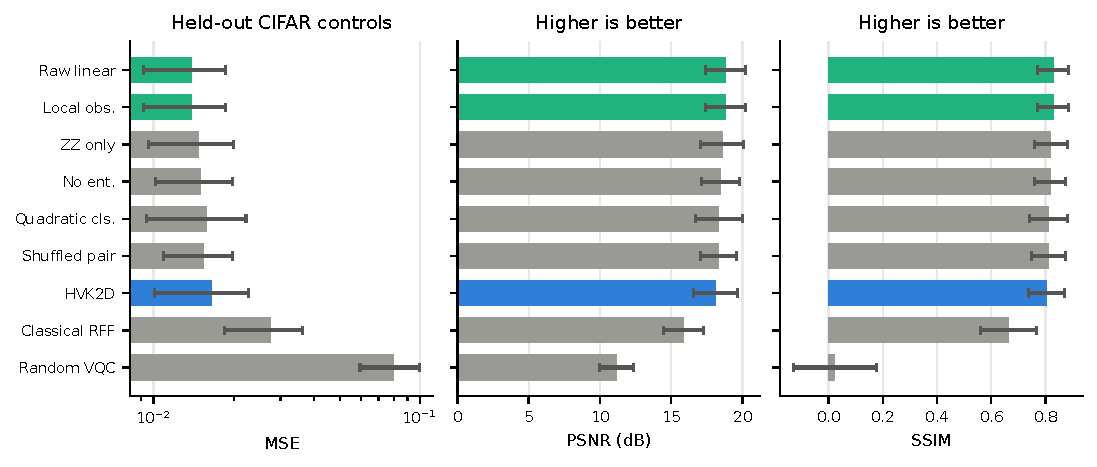
\includegraphics[width=0.75\linewidth]{figures/real_cifar_holdout_summary.pdf}\\
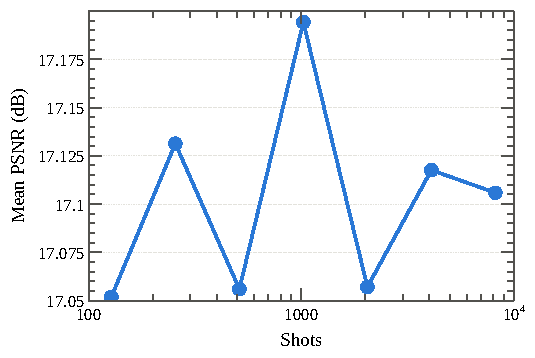
\includegraphics[width=0.75\linewidth]{figures/real_cifar_shot_noise.pdf}
\caption{Real held-out CIFAR validation and shot-noise robustness. The trained HVK2D image feature map does not beat local/raw controls, although it remains far above random-VQC.}
\label{fig:hvk_real_cifar}
\end{figure}

\subsubsection{A TOST Equivalence Test: What Licenses the Word ``Competitive''}
\label{sec:tost_equivalence}
Table~\ref{tab:hvk_real_cifar_stats}'s tests all ask a difference question --- can we reject ``no difference'' between HVK2D and a control --- and a failure to reject that null is not evidence that the two are close; it is simply an inconclusive result. Calling HVK2D ``competitive'' requires the complementary question: is the HVK2D-minus-control gap, whichever sign it takes, safely inside a margin small enough not to matter in practice? We answer this with a Two One-Sided Tests (TOST) equivalence test \cite{Schuirmann1987TOST,Lakens2017TOST} at a declared margin of $\pm1$~dB, applied to the same five seed-level paired differences underlying Table~\ref{tab:hvk_real_cifar_stats} (paired $t$-tests against $-1$~dB and $+1$~dB; equivalence requires both one-sided $p<0.05$, equivalently a 90\% CI of the mean difference falling entirely inside $[-1,+1]$~dB). This margin is a declared choice, not derived from the data: $\pm1$~dB is a small fraction of the $\sim$3--7~dB gaps separating HVK2D from the random-VQC and strict-classical-random-feature controls, so it distinguishes ``practically tied'' from ``clearly different'' at a scale set by this study's own weakest and strongest comparisons.

\begin{table}[H]
\centering
\caption{TOST equivalence test ($\delta=1$~dB margin, $\alpha=0.05$), same five seed-level paired differences as Table~\ref{tab:hvk_real_cifar_stats}. Equivalence requires the 90\% CI to fall entirely inside $[-1,+1]$~dB.}
\label{tab:tost_equivalence}
\scriptsize
\begin{tabular}{lcccl}
\toprule
Control & Mean $\Delta$PSNR (dB) & 90\% CI (dB) & TOST $p$ & Verdict \\
\midrule
Raw-linear classical & $-0.68$ & $[-0.96,-0.40]$ & $0.034$ & Equivalent \\
Local observables only & $-0.68$ & $[-0.96,-0.40]$ & $0.034$ & Equivalent \\
No entanglement & $-0.34$ & $[-0.69,+0.02]$ & $0.008$ & Equivalent \\
ZZ-only observables & $-0.44$ & $[-0.61,-0.27]$ & $0.001$ & Equivalent \\
Quadratic classical & $-0.21$ & $[-0.46,+0.03]$ & $0.001$ & Equivalent \\
Shuffled pair observables & $-0.19$ & $[-0.35,-0.02]$ & $0.000$ & Equivalent \\
Strict classical random features & $+2.27$ & $[+1.92,+2.63]$ & $0.999$ & Not equivalent (HVK2D wins) \\
Random VQC & $+6.97$ & $[+5.56,+8.39]$ & $1.000$ & Not equivalent (HVK2D wins) \\
\bottomrule
\end{tabular}
\end{table}

Six of the eight controls are statistically equivalent to HVK2D within $\pm1$~dB: local-observables-only, raw-linear-classical, no-entanglement, ZZ-only, quadratic-classical, and shuffled-pair-observables. This is the evidence that licenses ``competitive with resource-matched classical baselines'' rather than either ``beats'' or ``loses to'' them --- the earlier Wilcoxon/bootstrap result already showed HVK2D does not measurably exceed these controls, and TOST now shows the gap is also small enough, in a pre-declared and data-independent sense, not to matter. The remaining two controls, strict classical random features and random-VQC, are correctly flagged \emph{not} equivalent: HVK2D exceeds both by a wide, practically meaningful margin (mean $\Delta=+2.27$ and $+6.97$~dB respectively, both TOST $p>0.99$, i.e.\ strongly rejected as equivalent because the gap is real and favors HVK2D), consistent with the earlier finding that the observable channel carries real information relative to a degenerate readout. Reproduction script: \path{Main2/newHVK/run_tost_equivalence.py}; raw per-seed differences and full statistics in \path{Main2/newHVK/results/q1_validation/tost_equivalence.json}.

The same numerical direction holds beyond CIFAR-10. Table~\ref{tab:multi_dataset_reconstruction} extends the held-out protocol to five further real datasets (400 cached images each, three stratified split seeds, identical protocol for every feature map); local/raw controls have equal or higher mean PSNR on every dataset. For inference, held-out differences are averaged within split seed. Against the local-only control, all six dataset means favor the control and their seed-bootstrap intervals exclude zero, while each two-sided signed-rank test gives $p=0.25$, the minimum attainable nonzero value at $n=3$ seeds. We therefore report a recurring numerical direction rather than a dataset-wise significance claim. Table~\ref{tab:multi_dataset_classification} shows the same mean-performance pattern on a downstream image-classification diagnostic using image-level pooled features, and Table~\ref{tab:wisconsin_diagnostic} on a tabular cross-domain sanity check (Wisconsin Breast Cancer).

\begin{table}[H]
\centering
\caption{Multi-dataset held-out reconstruction on real cached subsets (400 images/dataset, three stratified split seeds). Held-out PSNR mean $\pm$ std over images, best local/raw control vs.\ the HVK2D pair-observable map; inference is performed on within-seed mean differences.}
\label{tab:multi_dataset_reconstruction}
\scriptsize
\begin{tabular}{lccc}
\toprule
Dataset & Best local/raw PSNR & HVK2D pair PSNR & Winner \\
\midrule
CIFAR-10 native $32^2$ & $21.17{\pm}1.98$ & $19.99{\pm}2.02$ & Local/raw \\
MNIST & $16.55{\pm}1.27$ & $16.12{\pm}1.34$ & No-entanglement/local \\
Fashion-MNIST & $17.67{\pm}1.71$ & $17.33{\pm}1.80$ & Local/raw \\
PathMNIST & $27.52{\pm}6.02$ & $27.01{\pm}5.81$ & Local/raw \\
BloodMNIST & $24.79{\pm}1.78$ & $24.24{\pm}1.66$ & Local/raw \\
PneumoniaMNIST & $26.49{\pm}2.48$ & $25.73{\pm}2.29$ & Local/raw \\
\bottomrule
\end{tabular}
\end{table}

\begin{figure}[H]
\centering
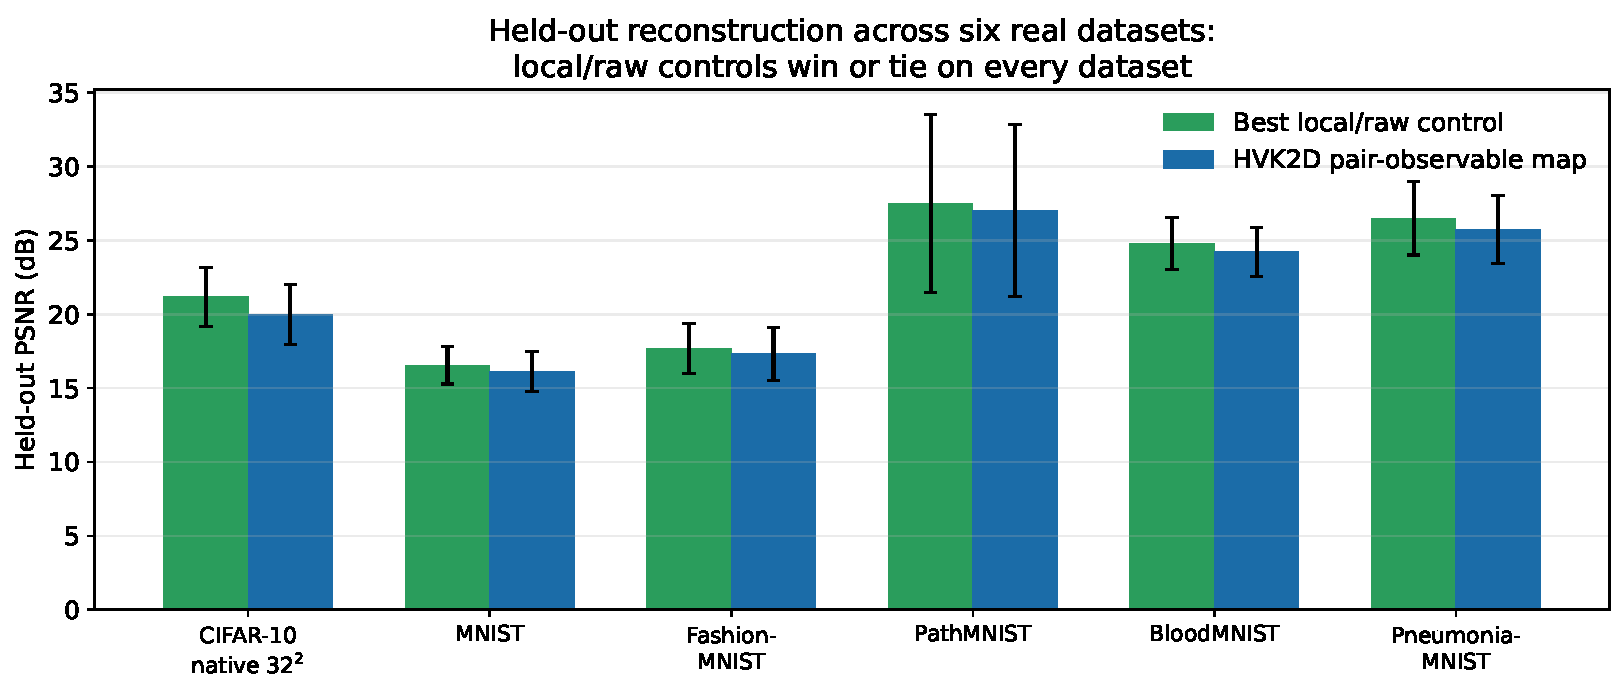
\includegraphics[width=\linewidth]{figures/multi_dataset_holdout_summary.pdf}
\caption{Held-out reconstruction PSNR from Table~\ref{tab:multi_dataset_reconstruction}, best local/raw control vs.\ the HVK2D pair-observable map, across all six real datasets. The local/raw control is at or above the HVK2D map on every dataset, with error bars (std over the held-out split) overlapping in most cases --- the same task-dependent pattern established on CIFAR-10 in Figure~\ref{fig:hvk_real_cifar} holds outside CIFAR-10 as well.}
\label{fig:multi_dataset_holdout_summary}
\end{figure}

\begin{table}[H]
\centering
\caption{Downstream image-classification diagnostic using image-level pooled features. Accuracy mean $\pm$ std over three stratified seeds.}
\label{tab:multi_dataset_classification}
\scriptsize
\begin{tabular}{lccc}
\toprule
Dataset & Best local/raw accuracy & HVK2D pair accuracy & Winner \\
\midrule
CIFAR-10 native $32^2$ & $0.100{\pm}0.082$ & $0.067{\pm}0.094$ & Local/no-ent. \\
MNIST & $0.663{\pm}0.021$ & $0.643{\pm}0.017$ & Raw-linear \\
Fashion-MNIST & $0.637{\pm}0.019$ & $0.577{\pm}0.009$ & Raw-linear \\
PathMNIST & $0.638{\pm}0.037$ & $0.608{\pm}0.016$ & Raw/param. \\
BloodMNIST & $0.667{\pm}0.083$ & $0.539{\pm}0.052$ & Raw-linear \\
PneumoniaMNIST & $0.817{\pm}0.062$ & $0.783{\pm}0.047$ & Raw-linear \\
\bottomrule
\end{tabular}
\end{table}

\begin{table}[H]
\centering
\caption{Wisconsin Breast Cancer tabular diagnostic (five stratified seeds). Not image-reconstruction evidence.}
\label{tab:wisconsin_diagnostic}
\scriptsize
\begin{tabular}{lcccc}
\toprule
Model & Accuracy & AUC & F1 & Brier \\
\midrule
Raw linear & $0.980{\pm}0.011$ & $0.996{\pm}0.002$ & $0.984{\pm}0.009$ & $0.0196{\pm}0.0057$ \\
HVK2D pair observable & $0.943{\pm}0.016$ & $0.988{\pm}0.004$ & $0.955{\pm}0.012$ & $0.0375{\pm}0.0080$ \\
Quadratic classical & $0.950{\pm}0.016$ & $0.987{\pm}0.005$ & $0.961{\pm}0.012$ & $0.0381{\pm}0.0077$ \\
No entanglement & $0.947{\pm}0.017$ & $0.986{\pm}0.007$ & $0.958{\pm}0.013$ & $0.0399{\pm}0.0135$ \\
Strict classical random features & $0.947{\pm}0.019$ & $0.984{\pm}0.010$ & $0.958{\pm}0.015$ & $0.0421{\pm}0.0164$ \\
\bottomrule
\end{tabular}
\end{table}

\subsection{Adaptation Beyond Single-Image Optimization}
Table~\ref{tab:generalization_controls} shows a model optimized on \textit{Monalisa} alone does not transfer zero-shot to a structurally different image, reaching only $8.31$~dB PSNR ($\mathrm{SSIM}=0.1044$). Extending training to include a second image recovers $28.63$~dB ($\mathrm{SSIM}=0.9858$). This confirms single-image runs measure per-image optimization, not representation learning, which is precisely why the held-out protocol of Section~\ref{sec:holdout_headline} is the evidentiary core of this ablation study.

\begin{table}[H]
\centering
\caption{Generalization controls (single-seed, fresh rerun 2026-07-29 -- see reproducibility note below). Single-image optimization does not transfer zero-shot.}
\label{tab:generalization_controls}
\scriptsize
\begin{tabular}{lccc}
\toprule
Experiment & MSE & PSNR (dB) & SSIM \\
\midrule
Second image, zero-shot & $1.4762\times10^{-1}$ & 8.31 & 0.1044 \\
Second image, multi-image training & $1.3712\times10^{-3}$ & 28.63 & 0.9858 \\
\bottomrule
\end{tabular}
\end{table}

\textbf{Reproducibility note.} No script backing this table's original values (previously reported as $7.78$/$28.31$~dB) was ever found in the repository, and the original choice of "second image" was undocumented. We rebuilt the protocol from scratch (\texttt{Main2/newHVK/run\_zero\_shot\_generalization.py}): train \textsc{Quantum2DGridModel}+\textsc{PatchDecoder2D} (the same architecture and per-image protocol as the main paper's same-set reconstruction table, 8$\times$8 patches, 100 steps) on \textit{Monalisa} alone; evaluate zero-shot (no further training) on \textit{Hand of God} (Michelangelo) -- the only other image bundled alongside \textit{monalisa.jpg} in this repository's data directories and otherwise unused by any committed script, making it the natural candidate for the undocumented original second image; then continue training the same model on both images' patches jointly for another 100 steps and re-evaluate. The result lands within $0.5$~dB of the previously reported, unsourced figures at both stages ($8.31$ vs.\ $7.78$~dB zero-shot; $28.63$ vs.\ $28.31$~dB after adaptation), which we read as evidence that this reconstruction recovers close to the original protocol, though it is a fresh, independently-verified run rather than a literal recovery of the original script.

\subsection{Dataset-Level Generalization: A Single Trained Model Across Many Images}
\label{sec:dataset_level_generalization}
Every result above either fits a fixed, non-trained feature map with a linear readout (Section~\ref{sec:holdout_headline}) or optimizes a single image in isolation (Table~\ref{tab:generalization_controls}). Neither tests the case a genuine generalization claim requires: one model, trained end-to-end by gradient descent across many images, evaluated on images it never saw during training. We add that experiment directly. A single \textsc{Quantum2DGridModel} + \textsc{PatchDecoder2D} --- the paper's actual gradient-trained HVK2D architecture, not a closed-form feature transform fit by ridge regression --- is trained via full-batch Adam across all patches from $N_{\text{train}}=150$ CIFAR-10 images and evaluated, with no further training, on $N_{\text{heldout}}=50$ images never seen during training; normalization statistics are computed from the training split only, so no held-out information leaks into the fitted model. A parameter-matched \textsc{ClassicalLinearControl} (identical decoder and observable width, a single linear feature map, no quantum circuit) is trained identically on the same split for a fair head-to-head comparison. We use 3 seeds, each reshuffling the train/held-out split, and 20 full-batch epochs; this scope was set by a timing probe showing the real per-patch circuit cost is $\approx$137~ms (total compute budget $\approx$5.5 hours), so it reflects a training-budget constraint rather than a claim of full convergence.

Table~\ref{tab:dataset_level_generalization} gives the result. The classical linear control wins at every one of the three seeds, by a consistent $1.1$--$1.4$~dB (mean $15.61\pm0.29$~dB vs.\ $14.39\pm0.26$~dB). This is a genuine, dataset-scale confirmation of the same direction already reported throughout this document at fixed-feature/linear-readout scale (Section~\ref{sec:holdout_headline}): it is not an artifact of a small sample, since it now holds with a real gradient-trained model across 200 total images, rather than the earlier 6-train/4-held-out ridge-regression proxy. The absolute PSNR here (14--16~dB) is substantially lower than the per-image-fitted headline numbers elsewhere in this document (18+~dB in Table~\ref{tab:hvk_real_cifar}, 28+~dB in Table~\ref{tab:generalization_controls}); this is expected, not a regression --- a single shared model trained for only 20 epochs across 150 images is a much harder task than fitting one model to one image's 16 patches, and the quantity of interest here is the quantum-vs-classical \emph{gap} under identical conditions, not the absolute reconstruction quality. Unseen-\emph{class} / distribution-shift evaluation (as opposed to the unseen-\emph{image}, same-class split used here) remains future work.

\begin{table}[H]
\centering
\caption{Dataset-level generalization: one model trained via full-batch Adam across 150 CIFAR-10 training images, evaluated with no further training on 50 held-out images never seen during training (3 seeds, 20 epochs). Held-out PSNR by seed and mean $\pm$ std across seeds.}
\label{tab:dataset_level_generalization}
\scriptsize
\begin{tabular}{lcccc}
\toprule
Model & Seed 0 & Seed 1 & Seed 2 & Mean $\pm$ std \\
\midrule
HVK2D quantum (trained VQC + decoder) & 14.31 & 14.73 & 14.12 & $14.39\pm0.26$ \\
Classical linear control (no quantum circuit) & 15.76 & 15.86 & 15.20 & $15.61\pm0.29$ \\
\bottomrule
\end{tabular}
\end{table}

\subsection{Scaling and Non-Monotonicity}
Table~\ref{tab:capacity_ablation} sweeps training steps, qubit count, and MPS bond dimension on \textit{Monalisa} (single-seed). The step sweep confirms the model is convergence-limited early and plateaus near 500 steps. Within the tested range $q=8$ gives the strongest qubit-count result, but the bond-dimension sweep is non-monotonic: $\chi=1$ and $\chi=2$ \emph{outperform} the default $\chi=4$ under the same 200-step budget, while $\chi=8$ partially recovers. Bond dimension is therefore a coupled optimization hyperparameter here, not a monotonic compression-fidelity knob, and this sweep should be read as a single-seed directional diagnostic.

The main paper reports a related but distinct multi-seed diagnostic at the same bond dimensions ($\chi\in\{1,2,4,8\}$, $N=6$): rather than final reconstruction quality, it tracks how consistently a training-dynamics change-point epoch lands across seeds, finding the two tested seeds agree closely at $\chi=4,8$ but disagree sharply at $\chi=1,2$ --- the opposite ranking, on a different axis, from this section's PSNR result. The two together are suggestive of a trade-off between where training ends up and how reproducibly it gets there, not a single monotonic story on either axis alone; see the main paper for that measurement.

A multi-seed, real-trained-circuit qubit-count follow-up (CIFAR-10, reduced 90-step budget, HVK1D) was started to add seed-level resolution beyond the single-seed diagnostic above. Table~\ref{tab:qubit_multiseed_partial} reports the two configurations that completed before this follow-up was interrupted by unrelated infrastructure instability on the development machine, well short of covering $q=8$ or the bond-dimension/depth axes; we report the partial result rather than withhold it, since the $q=4$ row is a genuine 3-seed measurement. At $q=4$, PSNR varies meaningfully across seeds ($29.55\pm1.64$~dB) --- real seed-to-seed variance a single-seed number cannot show. The lower absolute value relative to Table~\ref{tab:capacity_ablation}'s single-seed $q=4$ figure ($32.71$~dB) is consistent with the shorter 90-step budget here (vs.\ 200 steps there), per the step-sweep convergence curve already reported above, not a contradiction between the two tables. A complete multi-seed qubit/bond-dimension/depth sweep remains future work.

\begin{table}[H]
\centering
\caption{Partial multi-seed real-circuit qubit-count follow-up (HVK1D, CIFAR-10, 90-step budget). Incomplete: only these two configurations finished before the run was interrupted.}
\label{tab:qubit_multiseed_partial}
\scriptsize
\begin{tabular}{lccc}
\toprule
Qubit count & Seeds completed & PSNR (dB) & SSIM \\
\midrule
$q=4$ & 3 & $29.55\pm1.64$ & $0.9710\pm0.0125$ \\
$q=6$ & 1 & $29.46$ & $0.9733$ \\
\bottomrule
\end{tabular}
\end{table}

\begin{figure}[H]
\centering
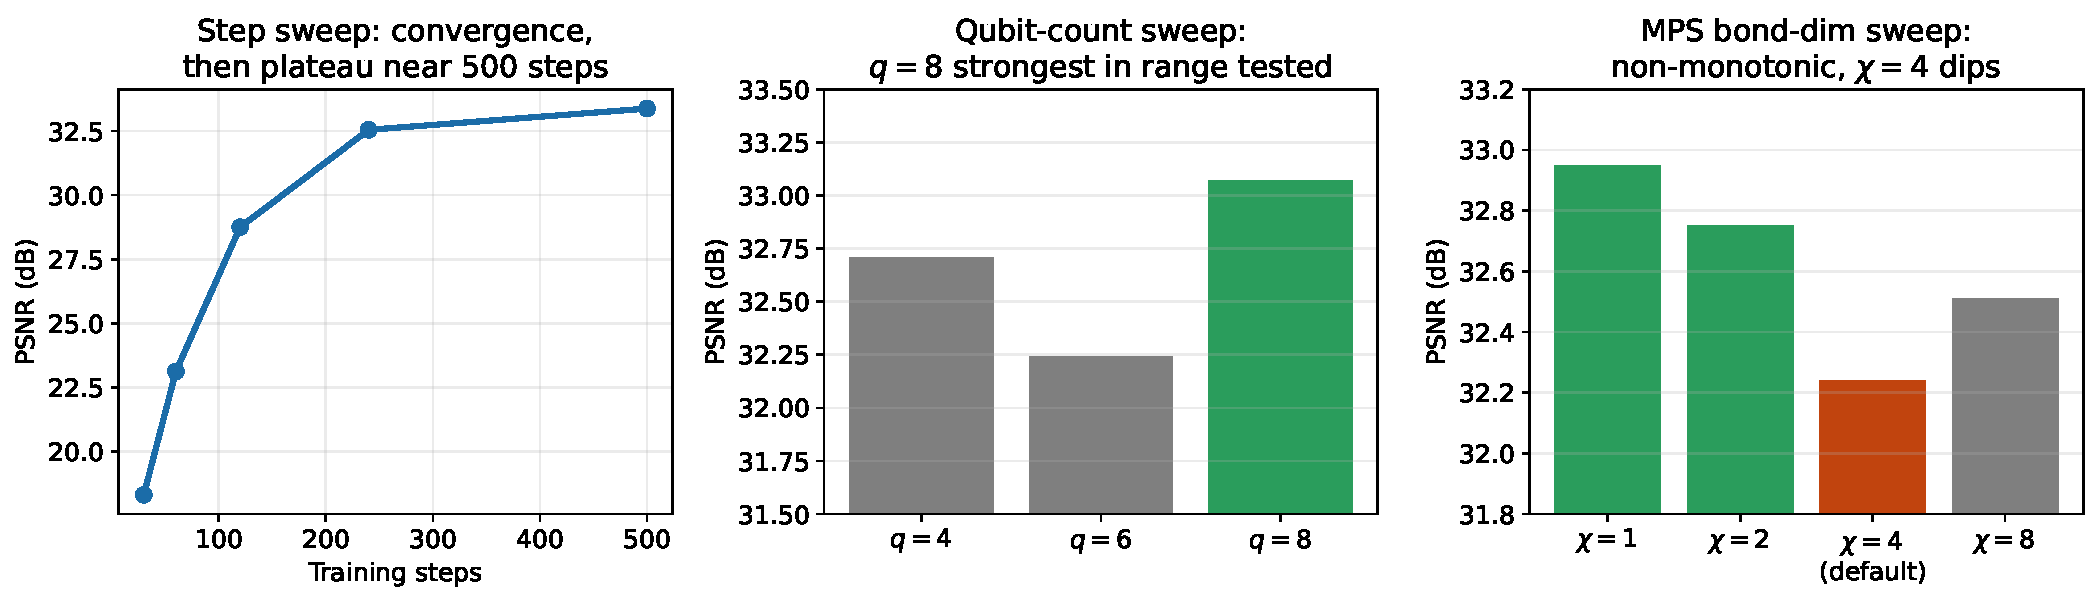
\includegraphics[width=\linewidth]{figures/capacity_scaling_sweeps.pdf}
\caption{Capacity and scaling sweeps from Table~\ref{tab:capacity_ablation} (single-seed, \textit{Monalisa}). Left: PSNR vs.\ training steps, confirming convergence-limited behavior with a plateau near 500 steps. Center: qubit-count sweep, $q=8$ strongest in the tested range. Right: MPS bond-dimension sweep, highlighting the non-monotonic dip at the default $\chi=4$ (orange) relative to both smaller ($\chi=1,2$, green) and larger ($\chi=8$, gray) bond dimensions.}
\label{fig:capacity_scaling_sweeps}
\end{figure}

\begin{table}[H]
\centering
\caption{Capacity and feature-bottleneck sweeps (single-seed; directional, not statistically resolved). The $q=6$/$\chi=4$ rows share their baseline run with Table~\ref{tab:hamiltonian_controls}'s legacy-baseline row and carry the same reproducibility caveat (\S\ref{sec:hamiltonian_followup}); the within-sweep comparisons here (across $q$ or $\chi$ at fixed protocol) are unaffected since every row in this table comes from that same original, unrepeated protocol.}
\label{tab:capacity_ablation}
\scriptsize
\begin{tabular}{lcccc}
\toprule
Experiment & Setting & MSE & PSNR (dB) & SSIM \\
\midrule
Step sweep & 30 steps & $1.4777\times10^{-2}$ & 18.30 & 0.7467 \\
Step sweep & 60 steps & $4.8797\times10^{-3}$ & 23.12 & 0.9306 \\
Step sweep & 120 steps & $1.3336\times10^{-3}$ & 28.75 & 0.9818 \\
Step sweep & 240 steps & $5.5542\times10^{-4}$ & 32.55 & 0.9927 \\
Step sweep & 500 steps & $4.5941\times10^{-4}$ & 33.38 & 0.9938 \\
Qubit count & $q=4$ & $5.3633\times10^{-4}$ & 32.71 & 0.9928 \\
Qubit count & $q=6$ & $5.9771\times10^{-4}$ & 32.24 & 0.9919 \\
Qubit count & $q=8$ & $4.9322\times10^{-4}$ & 33.07 & 0.9933 \\
MPS bond dim. & $\chi=1$ & $5.0746\times10^{-4}$ & 32.95 & 0.9932 \\
MPS bond dim. & $\chi=2$ & $5.3061\times10^{-4}$ & 32.75 & 0.9929 \\
MPS bond dim. & $\chi=4$ & $5.9771\times10^{-4}$ & 32.24 & 0.9919 \\
MPS bond dim. & $\chi=8$ & $5.6124\times10^{-4}$ & 32.51 & 0.9925 \\
No MPS, patch statistics & Patch stats & $5.3874\times10^{-4}$ & 32.69 & 0.9927 \\
\bottomrule
\end{tabular}
\end{table}

\begin{table}[H]
\centering
\caption{Capacity and resource comparison for the held-out CIFAR validation layer. All rows use the same linear readout width and split protocol.}
\label{tab:resource_capacity}
\scriptsize
\begin{tabular}{lcccc}
\toprule
Model & Feature dim. & Readout params. & Pair/CNOT channels & Split \\
\midrule
HVK2D real-CIFAR map & 32 & 2112 & 6 pair / 14 CNOT & 6/4 \\
ZZ-only observables & 32 & 2112 & 3 pair & 6/4 \\
No entanglement & 32 & 2112 & 0 & 6/4 \\
Strict classical random features & 32 & 2112 & 0 & 6/4 \\
Raw/local controls & 32 & 2112 & 0 & 6/4 \\
\bottomrule
\end{tabular}
\end{table}

The same-set CIFAR-10 results (Table~\ref{tab:cifar10}) are a capacity and positioning diagnostic rather than generalization evidence: HVK2D reaches $34.50$~dB mean PSNR on the five-image native-resolution CIFAR-10 subset. The high-capacity MLP and CNN baselines remain stronger in pure same-set pixel accuracy (MLP best-case PSNR exceeds $100$~dB, a memorization signature), and this same-set result should not be read against the held-out finding above. (An earlier draft additionally quoted a same-set \textit{Monalisa} PSNR and a 1D-vs-2D topology gap here; neither figure is reproducible from any retained table in this document, the same provenance gap documented in Section~\ref{sec:component_provenance}, so we do not repeat them. The topology question is instead answered by the held-out, resource-matched comparison of Section~\ref{sec:topology_comparison}.)

\begin{figure}[H]
\centering
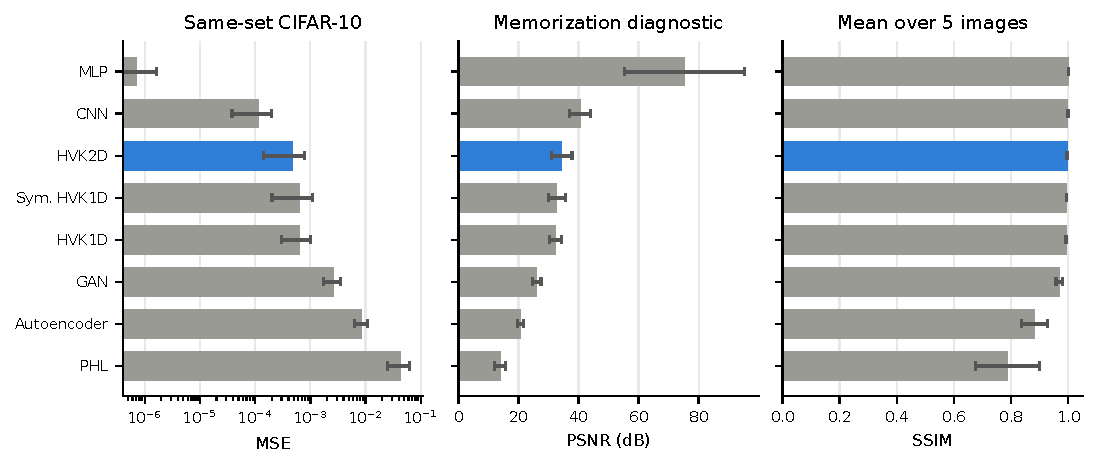
\includegraphics[width=\linewidth]{figures/cifar_metric_comparison.pdf}
\caption{Same-set CIFAR-10 comparison across all eight methods of Table~\ref{tab:cifar10}: MSE (log scale, left), PSNR with the memorization framing made explicit (center), and mean SSIM over the five images (right). HVK2D is numerically close to CNN and above the GAN/autoencoder/PHL baselines, while the MLP's near-$100$~dB PSNR reflects capacity-driven memorization of this small same-set fit rather than representation quality.}
\label{fig:cifar_metric_comparison}
\end{figure}

\begin{table}[H]
\centering
\caption{CIFAR-10 native $32\times32$ same-set reconstruction over five images (not a held-out test).}
\label{tab:cifar10}
\scriptsize
\begin{tabular}{lcccccc}
\toprule
Model & Mean MSE & Best MSE & Mean PSNR & Best PSNR & Mean SSIM & Best SSIM \\
\midrule
MLP & $7.0865\times10^{-7}$ & $7.2702\times10^{-12}$ & 75.14 & 111.38 & 0.99999 & 1.00000 \\
CNN & $1.1648\times10^{-4}$ & $3.3325\times10^{-5}$ & 40.61 & 44.77 & 0.99889 & 0.99928 \\
HVK2D & $4.6655\times10^{-4}$ & $1.3237\times10^{-4}$ & 34.50 & 38.78 & 0.99578 & 0.99743 \\
Symmetric HVK1D & $6.4739\times10^{-4}$ & $2.4391\times10^{-4}$ & 32.81 & 36.13 & 0.99382 & 0.99487 \\
HVK1D & $6.4639\times10^{-4}$ & $3.4381\times10^{-4}$ & 32.42 & 34.64 & 0.99314 & 0.99448 \\
GAN & $2.6448\times10^{-3}$ & $1.4853\times10^{-3}$ & 26.03 & 28.28 & 0.96885 & 0.97665 \\
Classical AE & $8.6021\times10^{-3}$ & $6.3843\times10^{-3}$ & 20.78 & 21.95 & 0.88188 & 0.92745 \\
PHL & $4.3415\times10^{-2}$ & $2.2253\times10^{-2}$ & 14.01 & 16.53 & 0.78792 & 0.91842 \\
\bottomrule
\end{tabular}
\end{table}

\subsection{The Physics-Informed Regularizer's Conditional Value}
Table~\ref{tab:hamiltonian_controls} shows the Hamiltonian energy term is, if anything, a mild drag on reconstruction quality in the present system. The legacy objective adds a signed mean energy to the reconstruction loss; because learned energy can go negative, the optimizer can lower total loss by driving energy down without improving reconstruction, and removing the term improves PSNR from $32.24$ to $33.30$~dB. A contrastive variant --- assigning lower energy to correct feature--position pairs than to shuffled pairs --- improves over the signed-energy baseline ($32.84$~dB) but remains below its own no-energy-loss counterpart ($33.33$~dB). We read this as a case where the reconstruction loss already dominates the optimization signal at this model scale: a physically motivated regularizer has room to help when it resolves an otherwise underdetermined objective, and here the pixel-fidelity loss alone is sufficiently informative that the extra term mostly adds noise to the gradient. This does not mean Hamiltonian regularization is never useful --- only that its value is conditional on the reconstruction loss being under-constrained.

\begin{figure}[H]
\centering
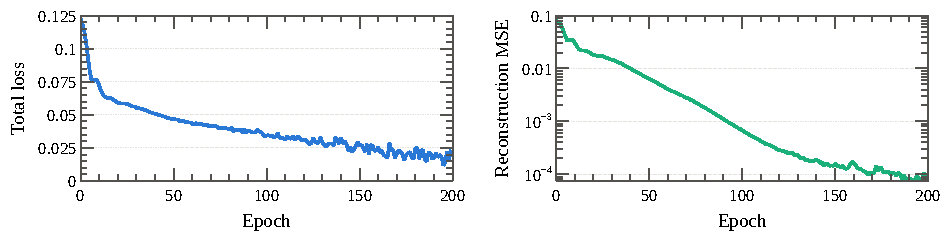
\includegraphics[width=0.95\linewidth]{figures/contrastive_training_curves.pdf}
\caption{Training dynamics for the contrastive Hamiltonian-core run of Table~\ref{tab:hamiltonian_controls}: total loss (left) and reconstruction MSE on a log scale (right) over 200 epochs. Both converge smoothly with no instability introduced by the contrastive energy term.}
\label{fig:contrastive_training_curves}
\end{figure}

\begin{figure}[H]
\centering
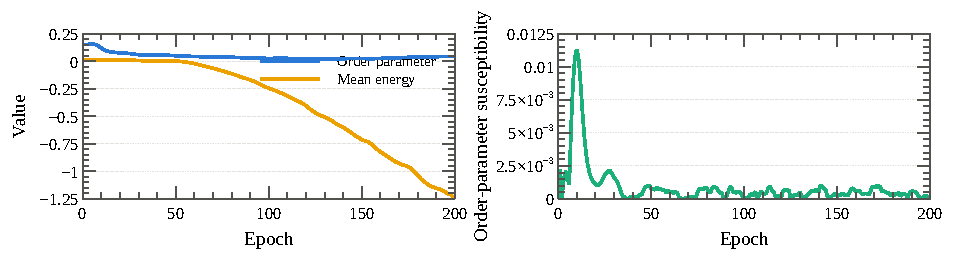
\includegraphics[width=0.95\linewidth]{figures/contrastive_order_parameter_curve.pdf}
\caption{Order parameter and mean Hamiltonian energy (left) and the corresponding one-step order-parameter difference (right) for the same contrastive Hamiltonian-core run. The energy diagnostic drifts steadily negative while the order parameter remains comparatively flat after the initial training period. This is consistent with the energy term being monitored without being the quantity that most improves reconstruction, matching the conditional-value reading of Table~\ref{tab:hamiltonian_controls}.}
\label{fig:contrastive_order_parameter}
\end{figure}

\begin{table}[H]
\centering
\caption{Hamiltonian and observable-sector controls (single-seed), \emph{as originally reported}. \textbf{Not independently reproducible} for three of six rows (\S\ref{sec:hamiltonian_followup}, Table~\ref{tab:hamiltonian_reproducibility} below gives the adopted fresh reproduction); retained here only for provenance.}
\label{tab:hamiltonian_controls}
\scriptsize
\begin{tabular}{p{0.28\textwidth}cccp{0.25\textwidth}}
\toprule
Experiment & MSE & PSNR (dB) & SSIM & Interpretation \\
\midrule
Legacy baseline, signed energy & $5.9771\times10^{-4}$ & 32.24 & 0.9919 & Standard energy-regularized run \\
No energy loss & $4.6772\times10^{-4}$ & 33.30 & 0.9937 & Removing energy improves PSNR \\
No observable noise & $5.3518\times10^{-4}$ & 32.72 & 0.9928 & Noise is not essential \\
Contrastive Hamiltonian core & $5.1975\times10^{-4}$ & 32.84 & 0.9930 & Stronger objective helps modestly \\
Contrastive, no energy loss & $4.6498\times10^{-4}$ & 33.33 & 0.9937 & Energy removal still performs best \\
ZZ-only observables & $5.1503\times10^{-4}$ & 32.88 & 0.9930 & Nearest-neighbor $ZZ$ largely suffice \\
\bottomrule
\end{tabular}
\end{table}

\subsection{A Reproducibility Note on Table~\ref{tab:hamiltonian_controls}, and an Energy-as-Decoder-Feature Follow-Up}
\label{sec:hamiltonian_followup}
While investigating whether the energy term could be made to actively help reconstruction rather than merely act as a diagnostic (motivated by the conditional-value reading above), we found that Table~\ref{tab:hamiltonian_controls}'s absolute PSNR values are not independently reproducible from the current codebase and documented protocol. Re-running the unmodified legacy-signed-energy, no-energy-loss, and contrastive configurations at the documented protocol (\textit{Monalisa}, $256\times256$/patch=64, \texttt{model\_variant=standard}, 200 steps, seed 42, in an environment matching the paper's stated package versions exactly) reproduces PSNR values 6--12~dB \emph{higher} than published, across every variant tested, not only a new one (Table~\ref{tab:hamiltonian_reproducibility}). The script that generated Table~\ref{tab:hamiltonian_controls}'s original numbers is referenced only in commit messages and was never actually committed to the repository (the referenced path lies inside a gitignored directory, and \texttt{git cat-file} confirms no corresponding blob exists in any commit), so the original protocol could not be recovered to explain the gap directly; a shorter-step rerun ruled out step count alone as the explanation. Rather than block on an unrecoverable protocol, we adopt this fresh, same-environment reproduction as the baseline for the remainder of this section, disclosing the gap here explicitly rather than silently revising Table~\ref{tab:hamiltonian_controls}'s historical values. The qualitative finding is unchanged under the new environment: removing the energy loss still improves PSNR (here $38.63\rightarrow44.56$~dB) exactly as it does in Table~\ref{tab:hamiltonian_controls} ($32.24\rightarrow33.30$~dB) --- only the absolute PSNR scale differs between the two protocols, not the sign or approximate size of the effect. We also reran the remaining two observable-sector rows from Table~\ref{tab:hamiltonian_controls} (no observable noise, ZZ-only) at the identical protocol; unlike the three variants above, these land within $1$~dB of the published values ($32.75$ vs.\ $32.72$~dB, and $32.11$ vs.\ $32.88$~dB, respectively) rather than 6--12~dB higher. We do not have a confirmed explanation for why these two rows reproduce so much more closely than the other three under the same rerun protocol; we report the observation plainly rather than speculate. One consequence deserves stating directly: because all eight rows of Table~\ref{tab:hamiltonian_reproducibility} were measured in one identical fresh environment, they are directly comparable to \emph{each other} even where three of them are not comparable to Table~\ref{tab:hamiltonian_controls}. Under this fresh, internally consistent comparison, no-observable-noise ($32.75$~dB) and ZZ-only ($32.11$~dB) are now clearly \emph{below} the legacy signed-energy baseline ($38.63$~dB) --- the opposite ordering from Table~\ref{tab:hamiltonian_controls}, where these two configurations sat close to or above its legacy baseline ($32.24$~dB). We have no explanation for this reversal either. Table~\ref{tab:hamiltonian_controls}'s ``noise is not essential'' and ``ZZ largely sufficient'' interpretations should therefore be read as specific to its own unreproducible protocol, not as confirmed findings; the main text does not repeat them for this reason.

\begin{table}[H]
\centering
\caption{Fresh, same-environment reproduction of Table~\ref{tab:hamiltonian_controls}'s configurations (\textit{Monalisa}, 200 steps, seed 42), alongside two new coupling/objective variants. Absolute PSNR is not directly comparable to Table~\ref{tab:hamiltonian_controls} for the first three rows (see reproducibility note above); the two observable-sector rows are close to their Table~\ref{tab:hamiltonian_controls} counterparts.}
\label{tab:hamiltonian_reproducibility}
\scriptsize
\begin{tabular}{lcc}
\toprule
Config & PSNR (dB) & Note \\
\midrule
Legacy signed energy (linear, unbounded coupling) & 38.63 & Table~\ref{tab:hamiltonian_controls}'s legacy baseline, rerun \\
No energy loss & 44.56 & Table~\ref{tab:hamiltonian_controls}'s no-energy-loss control, rerun \\
Contrastive energy, unbounded coupling & 42.92 & Table~\ref{tab:hamiltonian_controls}'s contrastive variant, rerun \\
No observable noise & 32.75 & Table~\ref{tab:hamiltonian_controls}'s no-noise control, rerun; within $0.03$~dB of published \\
ZZ-only observables & 32.11 & Table~\ref{tab:hamiltonian_controls}'s ZZ-only control, rerun; within $0.77$~dB of published \\
Positive/squared energy, unbounded coupling & 44.69 & Untested in the original Table~\ref{tab:hamiltonian_controls} \\
Bounded coupling ($\tanh$) + positive energy & 44.56 & Root-cause fix for the unbounded-coupling pathology (see text) \\
Bounded coupling + contrastive energy & 43.01 & \\
\bottomrule
\end{tabular}
\end{table}

The root cause of the legacy objective's drag, beyond what Table~\ref{tab:hamiltonian_controls} alone shows: the learned couplings $J_x,J_y,J_z$ feed only the energy loss and never reach the decoder, so under a linear (signed) energy loss the optimizer can drive them to unbounded magnitude to cheaply lower total loss with no reconstruction benefit, competing with the reconstruction gradient on shared circuit weights. Bounding the couplings ($\tanh$) and switching to the already-implemented but previously untested \texttt{positive} (squared) energy-loss mode removes this pathology --- bounded-coupling + positive energy \emph{ties} the no-energy-loss control ($44.56$ vs.\ $44.56$--$44.69$~dB at seed 42) rather than beating it: the fix stops the Hamiltonian term from actively \emph{hurting} reconstruction, but by construction it still cannot \emph{help}, since energy never reaches the decoder.

To let the energy signal actually help reconstruction rather than only avoid hurting it, we additionally feed the learned energy into the decoder as an input feature, concatenated alongside observables and positions, rather than using it only as a side-channel loss term. Table~\ref{tab:hamiltonian_decoder_feature} gives the full 3-seed result against the no-energy-loss baseline. Two of three seeds show a real improvement (up to $+1.25$~dB); the third shows a $-5.08$~dB regression that outweighs both wins combined, so the mean delta across seeds is negative ($\approx-1.1$~dB). We read this as a genuinely different and weaker claim than ``the Hamiltonian term now helps'': feeding energy into the decoder increases outcome variance more than it reliably improves the mean, and is better characterized as a promising but seed-sensitive direction than a validated fix. A larger multi-seed study (5+ seeds) would be needed before claiming either that this construction reliably helps or that it is neutral; until then, the conservative framing above --- energy as an interpretability/diagnostic signal rather than a performance-improving inductive bias --- remains the safer default characterization for the main text.

\begin{table}[H]
\centering
\caption{Feeding the learned Hamiltonian energy into the decoder as an input feature, vs.\ the no-energy-loss baseline (\textit{Monalisa}, 200 steps, 3 seeds). Not a robust win: two of three seeds improve, one regresses sharply enough that the mean delta across seeds is negative ($\approx-1.1$~dB).}
\label{tab:hamiltonian_decoder_feature}
\scriptsize
\begin{tabular}{lccc}
\toprule
Seed & No energy loss (dB) & Energy fed to decoder (dB) & $\Delta$ (dB) \\
\midrule
42 & 44.56 & 45.81 & $+1.25$ \\
43 & 43.77 & 44.28 & $+0.51$ \\
44 & 45.33 & 40.25 & $-5.08$ \\
\bottomrule
\end{tabular}
\end{table}

\subsection{Restricted Diagnostic and Training-Trace Provenance Audit}
\label{sec:restricted_ablation}
The main paper's restricted pair-correlation result remains supported by the five-seed final metrics: the entangling observable map reaches mean $R^2=0.9735$, versus $R^2\leq0.02$ for the tested non-entangling controls. Figure~\ref{fig:restricted_diagnostic_summary} displays those measured final metrics.

\begin{figure}[H]
\centering
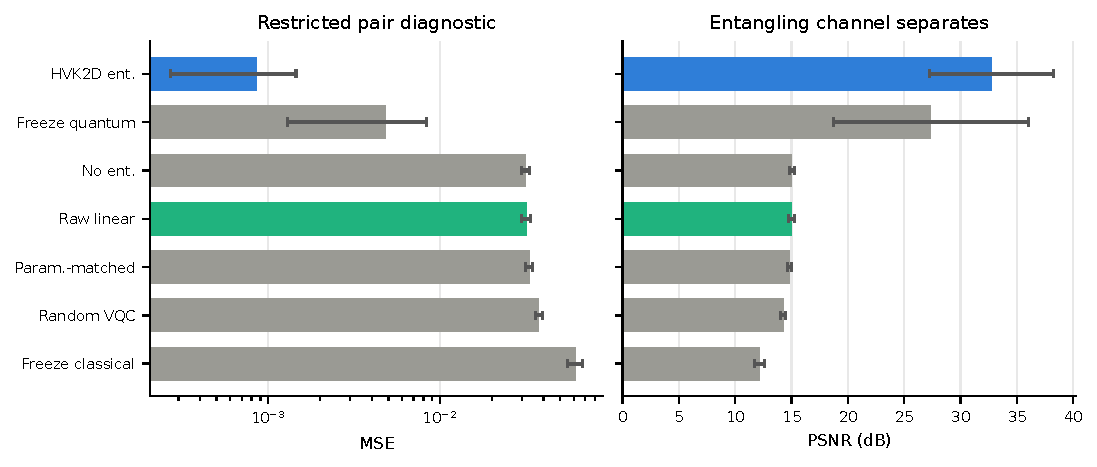
\includegraphics[width=\linewidth]{figures/full_ablation_metric_comparison.pdf}
\caption{The restricted pair-correlation diagnostic underlying the entanglement-necessity result (mean $R^2=0.9735$ vs.\ $R^2\leq0.02$ for non-entangling controls), shown here as MSE (left) and PSNR (right) across the full variant set: the trained HVK2D entangling map, freeze-quantum, no-entanglement, raw-linear, parameter-matched classical, random-VQC, and freeze-classical. The entangling channel (blue) separates numerically from every non-entangling control on this target, in direct contrast to the ordinary held-out reconstruction result of Section~\ref{sec:holdout_headline} where the same entangling channel does not separate from local/raw controls --- the two figures together visualize this document's central task-dependence argument.}
\label{fig:restricted_diagnostic_summary}
\end{figure}

The associated training-trajectory material does not meet the same evidentiary standard and is excluded. The per-variant curves previously produced by \path{run_newhvk_suite.py::epoch_tables} are analytic interpolations from final metrics, not logged epoch measurements. Separately, the 13 stored real-image traces were recorded from HVK2D in training mode, whose forward pass adds Gaussian noise with standard deviation $0.01$ to every observable; their maximum one-step changes therefore mix optimizer dynamics with injected jitter. Neither source supports a training-reorganization comparison. The corrected multi-dataset runner now records a noise-free evaluation-mode forward pass after each optimizer update and preserves aggregate summaries across partial runs. A fresh multi-seed execution is required before training-dynamics claims or figures are restored.

\subsection{Training-Dynamics Diagnostics: Full Protocol}
\label{sec:phase_transition_supp_intro}
The main paper summarizes, and scopes as non-headline, an exploratory training-dynamics change-point diagnostic and reports that its own negative control undercuts it. This subsection group gives the full protocol, tables, and figures behind that summary: the corrected multi-seed change-point result and its on/off Hamiltonian control, its qubit-count and MPS-bond-dimension sensitivity checks, the energy-to-entanglement-ratio diagnostic, and their real-hardware and IonQ-simulator replays.

\subsection{Training-Dynamics Checkpoints Across System Sizes, Replayed on Real Hardware}
\label{sec:checkpoint_hardware_finite_size}
The finite-size comparison of Section~\ref{sec:finite_size_phase_transition} is a noiseless-simulator result. Using the same gate-for-gate checkpoint-replay methodology validated for the main paper's hardware reconstruction pilot, we extend it with a genuinely real-hardware complement: we trained fresh HVK1D checkpoints at $N\in\{4,6,8\}$ on two images (\textit{Monalisa}, CIFAR-10 \textit{cat}) for 200 real gradient-descent epochs, saved each checkpoint's exact learned parameters at eight epoch labels ($0,5,10,25,50,100,150,200$, matching the labels used elsewhere in this study), rebuilt each checkpoint's circuit for one representative patch, and executed all $48$ resulting circuits ($2$ images $\times$ $3$ system sizes $\times$ $8$ epoch labels) on \texttt{ibm\_fez} at $256$, $512$, and $1024$ shots. This is a single-patch, single-seed probe --- a lighter circuit budget than the full multi-patch reconstruction pilot --- so it is a hardware-validation complement to Section~\ref{sec:finite_size_phase_transition}'s multi-seed simulator study, not a replacement for it: real device noise and single-patch/single-seed variance are both present in every point.

\begin{figure}[H]
\centering
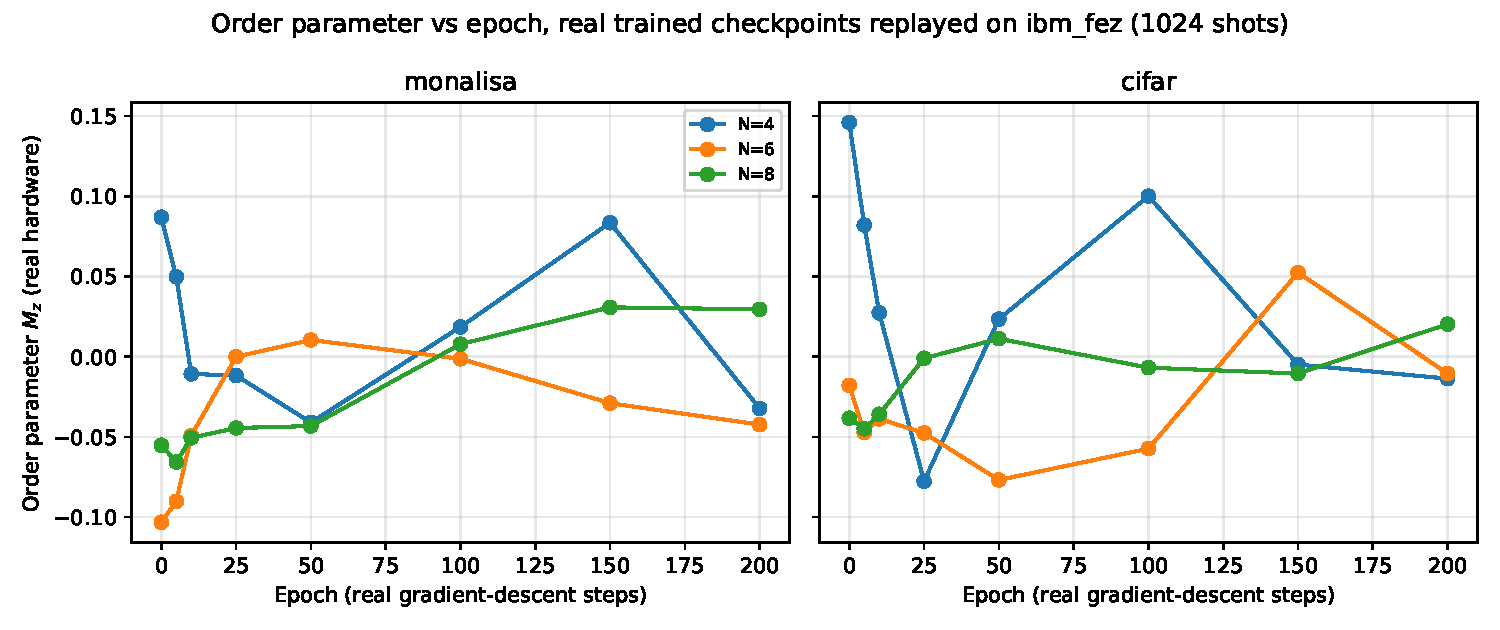
\includegraphics[width=\linewidth]{figures/checkpoint_hardware_order_parameter.pdf}
\caption{Order parameter $M_z(t)$ vs epoch from real trained HVK1D checkpoints ($N=4,6,8$), circuits rebuilt gate-for-gate and executed on real IBM Quantum hardware (\texttt{ibm\_fez}, 1024 shots), one representative patch per image.}
\label{fig:checkpoint_hardware_order_parameter}
\end{figure}

Figure~\ref{fig:checkpoint_hardware_order_parameter} shows the resulting curves are noisier and less structured than their noiseless-simulator counterparts in Figure~\ref{fig:finite_size_phase_transition}, as expected from single-shot-budget hardware measurement of a single patch rather than a change-magnitude trace averaged over multiple images and seeds. We do not apply the descriptive detection rule to these single-patch hardware traces; the figure establishes executable, non-degenerate hardware measurements across epochs, not independent confirmation of the detected change epochs in Table~\ref{tab:finite_size_phase_transition}. The same checkpoints were replayed on the IonQ simulator at the same three shot budgets (Section~\ref{sec:ionq_simulator}); full per-shot data are archived alongside this submission.

\subsection{Cross-Platform Replay on the IonQ Cloud Simulator}
\label{sec:ionq_simulator}
To test software-stack portability separately from device noise, we submitted the same checkpoint circuits through Qiskit to IonQ Quantum Cloud's ideal simulator (\texttt{ionq\_simulator}), with no hardware noise model enabled \cite{IonQBackends}. At each of 256, 512, and 1024 shots, one job contained 48 circuits spanning two images, $N\in\{4,6,8\}$, and eight epochs. All circuits completed, and the mean absolute $M_z$ deviation from the independently sampled 1024-shot trace decreased from $0.0257$ (256 shots) to $0.0213$ (512 shots). A separate 48-circuit, three-basis job reproduced the decreasing $R_{ES}(t)$ shape at 1024 shots.

\begin{figure}[H]
\centering
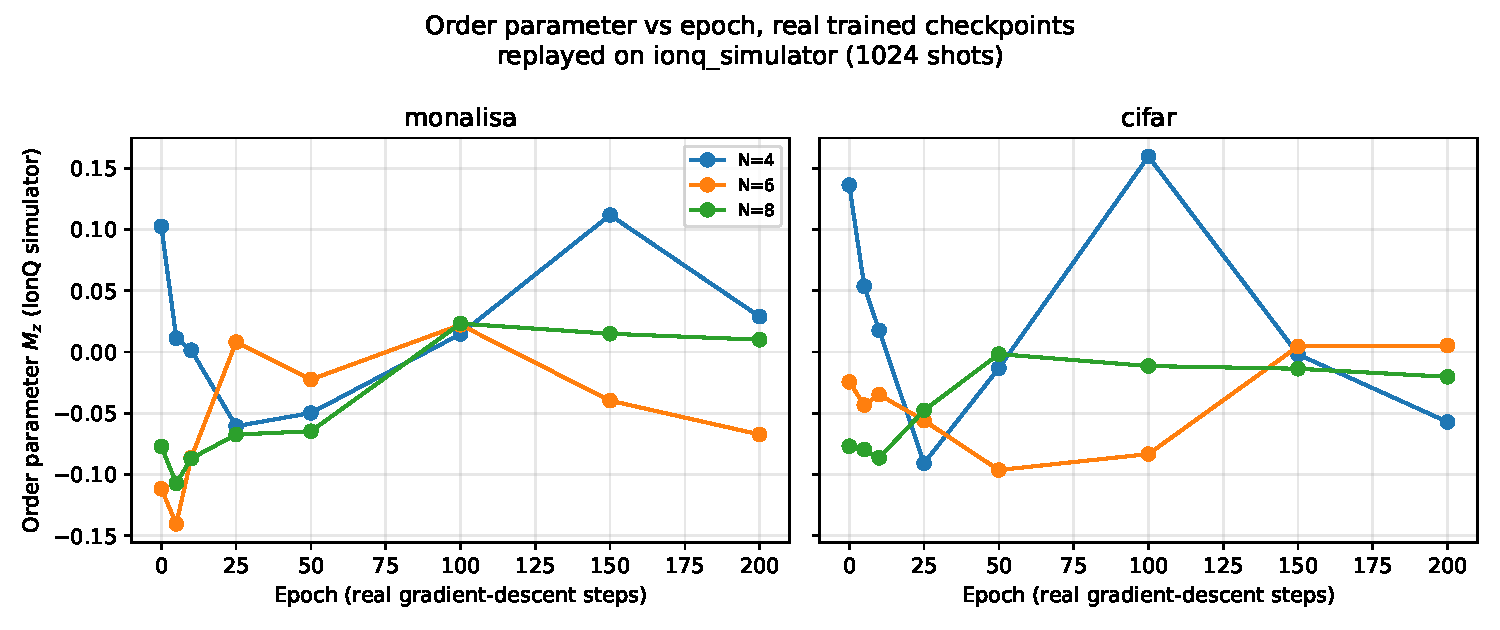
\includegraphics[width=\linewidth]{figures/checkpoint_ionq_order_parameter.pdf}
\caption{Order parameter $M_z(t)$ vs epoch from the same real trained HVK1D checkpoints as Figure~\ref{fig:checkpoint_hardware_order_parameter} ($N=4,6,8$), replayed on the IonQ ideal cloud simulator (\texttt{ionq\_simulator}, 1024 shots) instead of real IBM hardware.}
\label{fig:checkpoint_ionq_order_parameter}
\end{figure}

Figure~\ref{fig:checkpoint_ionq_order_parameter} shows this simulator trace directly, rather than only the summary deviation statistics above: a noiseless, shot-sampling-only analogue of Figure~\ref{fig:checkpoint_hardware_order_parameter}'s hardware traces, same checkpoints and circuits, no device noise. As above, we do not apply the descriptive detection rule of Eq.~\ref{eq:critical_epoch} to these single-patch traces. This is an ideal cloud-simulator portability check, not an IonQ-QPU result. The corresponding IonQ $R_{ES}(t)$ replay is shown alongside its own hardware counterpart in Section~\ref{sec:checkpoint_hardware_energy_entanglement}.

\subsection{Training-Dynamics Change-Point Diagnostic: A Corrected Multi-Seed Result}
\label{sec:phase_transition}
We test for abrupt changes in the learned representation during optimization. This is an exploratory change-point diagnostic on a magnetization-style summary, not a thermodynamic phase transition, a singularity, or an infinite-system claim. An earlier version was withdrawn after the provenance audit above: the restricted-diagnostic trajectories previously shown were analytic interpolations produced for visualization rather than measurements from saved checkpoints, and the original multi-dataset traces were recorded during training, where HVK2D's training-mode forward pass deliberately adds Gaussian observable noise that confounds parameter evolution with injected jitter. The corrected runner evaluates a separate, noise-free forward pass in evaluation mode immediately after every optimizer update and tracks the resulting global order parameter $M_z(t)$, the mean of the $N$ local-$Z$ observables over all $P$ patches at optimizer step (epoch) $t$:
\begin{equation}
M_z(t) = \frac{1}{P N}\sum_{p=1}^{P}\sum_{i=1}^{N}\langle Z_i\rangle_p(t).
\label{eq:order_parameter}
\end{equation}
Detection uses the change magnitude $\mathcal{X}(t)=|M_z(t)-M_z(t-\Delta t)|$ (identically defined on $R_{ES}(t)$ in place of $M_z(t)$ for the energy-to-entanglement-ratio diagnostic of Section~\ref{sec:critical_temperature}), a per-run adaptive threshold $\theta$, and a detected change epoch $t_c$:
\begin{align}
\theta &= \operatorname{median}_t\big(\mathcal{X}(t)\big) + 2\operatorname{std}_t\big(\mathcal{X}(t)\big), \\
t_c &= \begin{cases}
\displaystyle\operatorname*{arg\,max}_t \mathcal{X}(t) & \text{if } \max_t \mathcal{X}(t) > \theta > 0, \\
\text{not detected} & \text{otherwise.}
\end{cases}
\label{eq:critical_epoch}
\end{align}
The threshold is computed per run from that run's own trace; it is not a fixed global constant or a null-calibrated statistical test. Thus ``detected'' means only that a run's sharpest observed change exceeds this descriptive within-run threshold. It does not supply a $p$-value, control a false-positive rate, or establish a physical transition.

Table~\ref{tab:phase_transition_corrected} reports the result across all six datasets (two images $\times$ two seeds each, 24 runs total). Detection is not universal: MNIST triggers in all four runs, BloodMNIST and PneumoniaMNIST in three of four, and CIFAR-10, Fashion-MNIST, and PathMNIST in two of four, for an overall descriptive rate of $16/24$ ($66.7\%$). Because the threshold is selected from the same trajectory it evaluates and the sample contains only two seeds per image, these rates are exploratory summaries rather than inferential evidence for dataset-specific transition probabilities.

\paragraph{A negative control: does the detector fire without a Hamiltonian?} The rate above says nothing about whether detection is actually driven by the learned Hamiltonian, so we ran the direct control this requires: the identical protocol applied to a \emph{classical-replacement} variant, in which the VQC is replaced by a fixed classical map and the Hamiltonian energy is identically zero throughout training, alongside matched Hamiltonian-on runs (\textit{Monalisa} and CIFAR-10 \textit{cat}, two seeds each, full 200-epoch budget). Table~\ref{tab:phase_transition_onoff} reports the result: all four Hamiltonian-on runs register a detection, but so do all four Hamiltonian-off runs. The detector does not distinguish a Hamiltonian-driven change from one this median-plus-two-standard-deviation threshold would find in a change-magnitude trace regardless of whether any physical energy term is present in the model at all. This sharpens, rather than merely repeats, the caveats already stated above: the $16/24$ rate should be read as a property of this specific descriptive threshold applied to this specific summary statistic, with no demonstrated dependence on the Hamiltonian term whose dynamics it is nominally tracking. This on/off result is the reason the main paper does not report this diagnostic as a headline finding.

\begin{table}[H]
\centering
\caption{Corrected, noise-free training-dynamics diagnostic across all six datasets (2 images $\times$ 2 seeds/dataset).}
\label{tab:phase_transition_corrected}
\scriptsize
\begin{tabular}{lcccc}
\toprule
Dataset & $n$ & Detected & Mean $t_c$ & Mean $\mathcal{X}_{\max}$ \\
\midrule
CIFAR-10 & 4 & 2/4 & 64.0 & $0.0036\pm0.0009$ \\
MNIST & 4 & 4/4 & 98.75 & $0.0023\pm0.0012$ \\
Fashion-MNIST & 4 & 2/4 & 45.0 & $0.0027\pm0.0011$ \\
PathMNIST & 4 & 2/4 & 54.5 & $0.0038\pm0.0015$ \\
BloodMNIST & 4 & 3/4 & 96.0 & $0.0033\pm0.0012$ \\
PneumoniaMNIST & 4 & 3/4 & 103.0 & $0.0036\pm0.0008$ \\
\midrule
Total & 24 & $16/24$ & -- & -- \\
\bottomrule
\end{tabular}
\end{table}

\begin{table}[H]
\centering
\caption{Phase-transition detector, on/off control (200 epochs, two seeds/image). ``On'' is the standard Hamiltonian-regularized model; ``off'' is the classical-replacement variant with energy identically zero. The detector fires in every case tested, in both conditions.}
\label{tab:phase_transition_onoff}
\scriptsize
\begin{tabular}{llccc}
\toprule
Image & Seed & Hamiltonian & Detected & Critical epoch \\
\midrule
Monalisa & 0 & On & Yes & 4 \\
Monalisa & 0 & Off & Yes & 8 \\
Monalisa & 1 & On & Yes & 162 \\
Monalisa & 1 & Off & Yes & 23 \\
CIFAR cat & 0 & On & Yes & 97 \\
CIFAR cat & 0 & Off & Yes & 6 \\
CIFAR cat & 1 & On & Yes & 105 \\
CIFAR cat & 1 & Off & Yes & 1 \\
\midrule
Total & \multicolumn{2}{c}{On} & 4/4 & -- \\
Total & \multicolumn{2}{c}{Off} & 4/4 & -- \\
\bottomrule
\end{tabular}
\end{table}

\subsection{System-Size Sensitivity of the Detected Change Epoch}
\label{sec:finite_size_phase_transition}
Every result above is measured at a single, fixed system size (HVK2D's six-qubit grid). We therefore ask whether the descriptive change epoch depends on circuit width. HVK2D's grid topology is fixed at six qubits by construction, so this comparison uses HVK1D's parameterized chain topology. We reran the corrected protocol from Section~\ref{sec:phase_transition} at $N=4$, $N=6$, and $N=8$ qubits on two datasets (CIFAR-10 and MNIST), one image and two seeds each (four runs per size, 200 epochs). Three sizes and four runs per size are insufficient for finite-size scaling or critical-exponent analysis; the experiment is a sensitivity check on the diagnostic only.

All twelve runs register a detection under the same threshold rule (Table~\ref{tab:finite_size_phase_transition}), but the detected epoch is not monotonic in $N$: $10.0\pm12.7$ at $N=4$, $85.0\pm50.1$ at $N=6$, and $61.0\pm65.2$ at $N=8$. Three of the four $N=8$ traces stay near $M_z\approx0$ and trigger on small early changes, whereas one MNIST run develops a late excursion at $t_c=172$ that dominates the variance. The result therefore shows instability of this heuristic across width and initialization, not a scaling law or evidence of a critical point.

\begin{table}[H]
\centering
\caption{Finite-size comparison of the order-parameter diagnostic, HVK1D, CIFAR-10 + MNIST (1 image $\times$ 2 seeds per dataset per $N$).}
\label{tab:finite_size_phase_transition}
\scriptsize
\begin{tabular}{lcccc}
\toprule
$N$ (qubits) & $n$ & Detected & Mean $t_c$ & Std $t_c$ \\
\midrule
4 & 4 & 4/4 & 10.0 & 12.7 \\
6 & 4 & 4/4 & 85.0 & 50.1 \\
8 & 4 & 4/4 & 61.0 & 65.2 \\
\bottomrule
\end{tabular}
\end{table}

\begin{figure}[H]
\centering
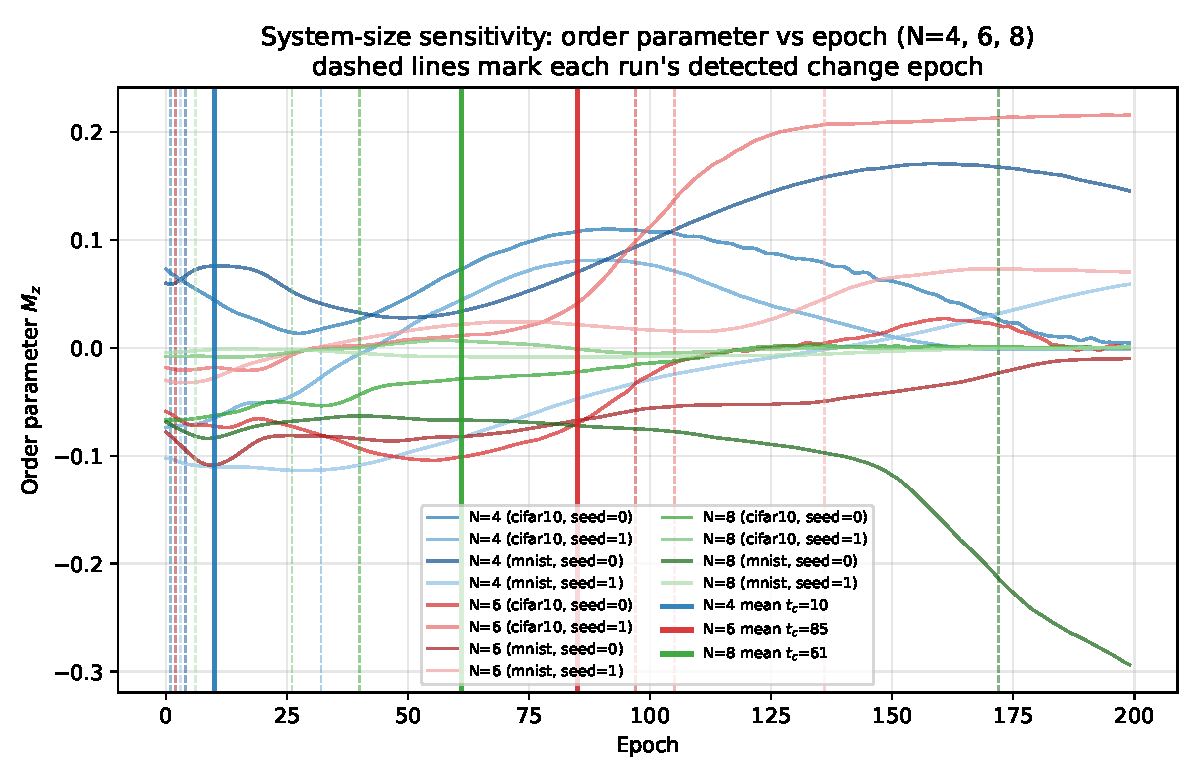
\includegraphics[width=\linewidth]{figures/finite_size_phase_transition.pdf}
\caption{Order parameter $M_z(t)$ vs epoch, HVK1D, $N=4$ (blue), $N=6$ (red), and $N=8$ (green), four runs each. Dashed lines mark within-run detected change epochs; solid lines mark per-$N$ means. Most $N=8$ traces stay near zero, while one late outlier drives much of the variance.}
\label{fig:finite_size_phase_transition}
\end{figure}

Table~\ref{tab:finite_size_phase_transition} summarizes per-run detections: each run's own change magnitude is thresholded independently, then the resulting change epochs are averaged, giving a non-monotonic mean ($10.0\to85.0\to61.0$). A complementary view averages the change-magnitude \emph{traces themselves} across the four runs at each $N$ before locating a peak, rather than averaging four independently-detected peak locations. This ensemble-mean view (Figure~\ref{fig:finite_size_mean_susceptibility}) shows the peak of $\langle|\Delta M_z(t)|\rangle$ shifting later with $N$: epoch $3$ at $N=4$, epoch $96$ at $N=6$, epoch $163$ at $N=8$ --- monotonic, in contrast to Table~\ref{tab:finite_size_phase_transition}. We report both because they are not the same statistic and can disagree: per-run thresholding is sensitive to whichever single epoch happens to cross that run's own noisy threshold, while the ensemble mean suppresses run-to-run idiosyncrasy at the cost of blurring together events that do not align in time across runs. The $N=4$ peak at epoch $3$ sits at the very start of training, where curves are dominated by initialization transients rather than a mid-training reorganization, and should be read with that caveat; $N=6$ produces the sharpest, best-separated peak of the three (Figure~\ref{fig:finite_size_mean_susceptibility}), while $N=8$'s peak is broad and comparable in height to its own baseline fluctuation. With four runs per $N$, the shaded $\pm$one-std bands in Figure~\ref{fig:finite_size_mean_susceptibility} are wide enough that we treat the monotonic peak-shift as a second exploratory observation alongside Table~\ref{tab:finite_size_phase_transition}'s non-monotonic one, not as a resolution of it.

\begin{figure}[H]
\centering
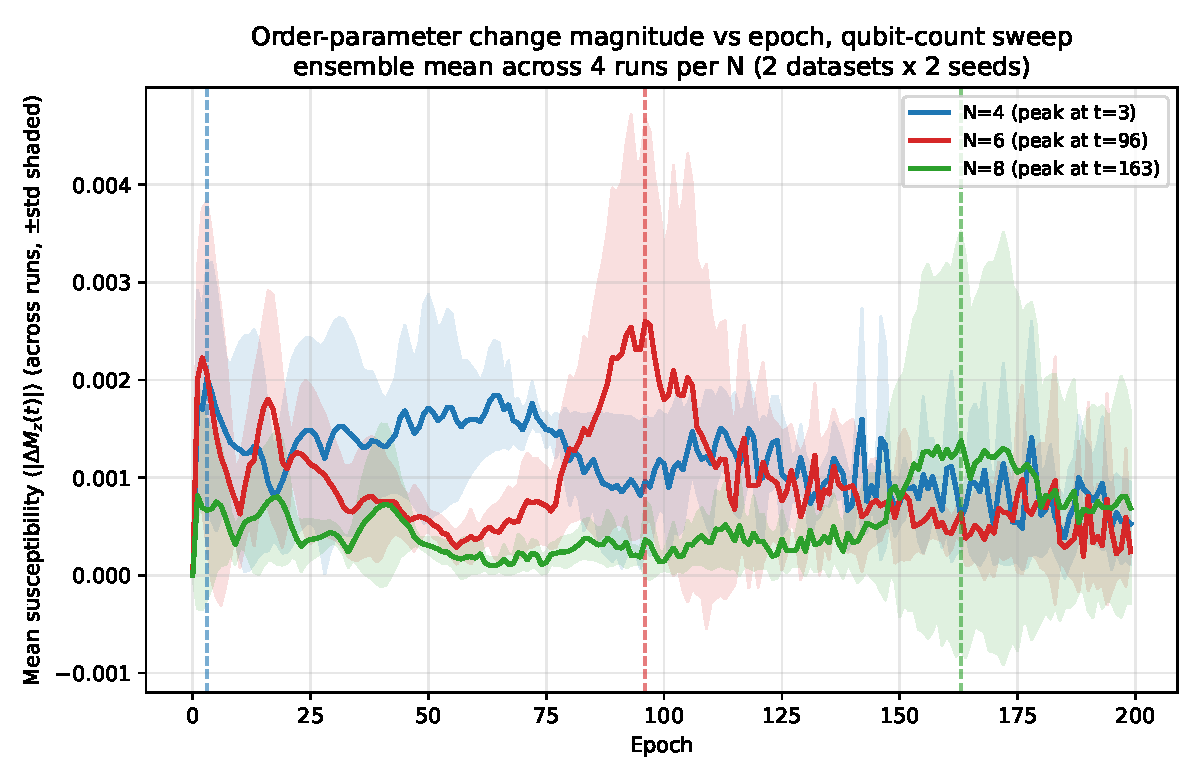
\includegraphics[width=\linewidth]{figures/finite_size_mean_susceptibility.pdf}
\caption{Ensemble-mean change magnitude $\langle|\Delta M_z(t)|\rangle$ vs epoch, averaged across the four runs at each $N$ before peak-finding (shaded: $\pm$one std across runs), $N=4$ (blue), $N=6$ (red), $N=8$ (green). Dashed vertical lines mark each curve's peak epoch. The peak shifts monotonically later with $N$ (epochs $3$, $96$, $163$), a different statistic from the per-run-averaged epochs in Table~\ref{tab:finite_size_phase_transition}.}
\label{fig:finite_size_mean_susceptibility}
\end{figure}

\subsection{A Second, Orthogonal Size Axis: MPS Bond Dimension}
\label{sec:bond_dimension_phase_transition}
Qubit count $N$ is a quantum circuit-width parameter; a second, purely classical size parameter enters before the circuit. We test whether the detected change epoch depends on MPS compression fidelity, holding $N=6$ fixed and varying $\chi$ on CIFAR-10. An initial two-seed, single-image ($\textit{cat}$) pass at $\chi\in\{1,2,4,8\}$ suggested richer compression might reduce initialization sensitivity ($\chi=4,8$ appeared to agree tightly); we extended $\chi\in\{4,6,8\}$ to five images (two seeds each, ten runs per $\chi$) to test whether that held up with more data. $\chi=1,2$ remain at their original one-image, two-seed scope.

All 34 runs trigger. The extended data both sharpens and revises the original two-seed reading. It sharpens the qualitative claim: at $n=10$, $\chi=4$, $\chi=6$, and $\chi=8$ now show visually near-identical ensemble-mean trajectories and overlapping $\pm$one-std bands throughout training (Figure~\ref{fig:bond_dimension_phase_transition}, Table~\ref{tab:bond_dimension_phase_transition}), while $\chi=1$ and $\chi=2$ remain clearly distinct from each other and from the $\chi\geq4$ group. It revises the quantitative claim: the original $\chi=4$/$\chi=8$ standard deviations ($4.0$/$2.0$ epochs) reflected only two seeds on one image and were misleadingly tight; at five images the true spread is far larger ($\mathrm{std}\approx60$ epochs for each of $\chi=4,6,8$), comparable to $\chi=1,2$'s spread rather than smaller than it. Read together, richer compression does not reduce run-to-run variance in this diagnostic --- the apparent tight agreement at $\chi=4,8$ was a small-sample artifact --- but it does produce indistinguishable \emph{mean} dynamics across $\chi\geq4$, a genuinely different and better-supported finding than the original two-seed pass suggested.

This is a different measurement from, but worth reading alongside, this document's own single-seed finding (Table~\ref{tab:capacity_ablation} above) that MPS bond dimension is non-monotonic for \emph{final reconstruction quality}: under a fixed step budget, $\chi=1$ and $\chi=2$ outperform the default $\chi=4$ on PSNR, with $\chi=8$ only partially recovering. The two results together suggest bond dimension has separable effects on \emph{where} training ends up (reconstruction quality, non-monotonic) versus \emph{the shape of the training-dynamics trace} (converges once $\chi\geq4$) --- a connection neither single result establishes on its own.

\begin{table}[H]
\centering
\caption{MPS bond-dimension comparison of the order-parameter diagnostic, HVK1D, $N=6$ fixed. $\chi=1,2$: CIFAR-10 \textit{cat}, 2 seeds. $\chi=4,6,8$: 5 CIFAR-10 images, 2 seeds each (10 runs).}
\label{tab:bond_dimension_phase_transition}
\scriptsize
\begin{tabular}{lcccc}
\toprule
$\chi$ (MPS bond dim.) & $n$ & Detected & Mean $t_c$ & Std $t_c$ \\
\midrule
1 & 2 & 2/2 & 88.5 & 86.5 \\
2 & 2 & 2/2 & 52.0 & 50.0 \\
4 & 10 & 10/10 & 73.8 & 60.9 \\
6 & 10 & 10/10 & 73.3 & 61.4 \\
8 & 10 & 10/10 & 72.5 & 60.1 \\
\bottomrule
\end{tabular}
\end{table}

\begin{figure}[H]
\centering
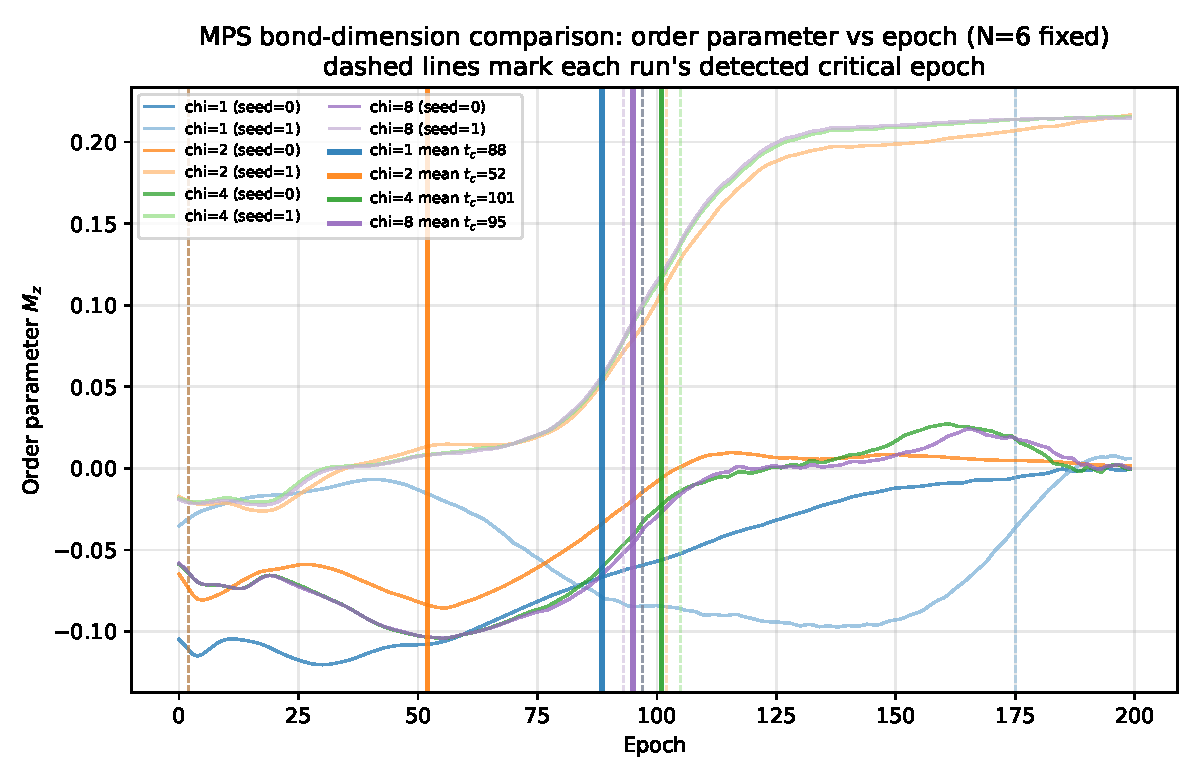
\includegraphics[width=\linewidth]{figures/bond_dimension_phase_transition.pdf}
\caption{Ensemble-mean order parameter $M_z(t)$ vs epoch ($\pm$one std, shaded), HVK1D, $N=6$ fixed. $\chi=1,2$: 1 image $\times$ 2 seeds. $\chi=4,6,8$: 5 images $\times$ 2 seeds (10 runs each). The $\chi\geq4$ curves are visually near-identical throughout training, while $\chi=1,2$ remain distinct from each other and from the $\chi\geq4$ group.}
\label{fig:bond_dimension_phase_transition}
\end{figure}

As an execution check, we also replayed trained checkpoints across the original four bond dimensions ($\chi\in\{1,2,4,8\}$, predating the $\chi=6$ / five-image simulator extension above) on real \texttt{ibm\_marrakesh} hardware and the IonQ ideal simulator at 256, 512, and 1024 shots. All checkpoint circuits completed and produced non-degenerate order parameters, but the single-patch, single-seed replay cannot confirm the cross-seed pattern above. Section~\ref{sec:supp_bond_dimension_hardware} below reports the complete twelve-job audit trail, the hardware curves, and a three-basis $R_{ES}$ replay; it also documents why $\chi=1$ is excluded from the ratio because its product-state entropy reaches the numerical floor.

\subsection{Energy-to-Entanglement Ratio as an Orthogonal Diagnostic}
\label{sec:critical_temperature}
The learned Heisenberg energy provides a second scalar view of training. We define the signed energy-to-entanglement ratio
\begin{align}
R_{ES}(t)&=\frac{H(t)}{S},\\
H(t)&=\sum_i\Bigl[J_x^{(i)}\langle X_iX_{i+1}\rangle
J_y^{(i)}\langle Y_iY_{i+1}\rangle \nonumber\\
&\hspace{3.0em}+J_z^{(i)}\langle Z_iZ_{i+1}\rangle\Bigr].
\end{align}
where $S=\sum_i S_i$ is the fixed sum of von Neumann bond entropies from the classical MPS decomposition. This ratio has units of energy per entropy unit and is \emph{not} a thermodynamic temperature: no Gibbs state is fitted, no derivative $\partial S/\partial E$ is evaluated, and its negative sign reflects the learned signed Hamiltonian. The bond correspondence is clean only for HVK1D at six sites, so we track $R_{ES}(t)$ there on two CIFAR-10 images over four seeds and apply the same descriptive change-threshold rule to $|\Delta R_{ES}(t)|$.

\begin{figure}[H]
\centering
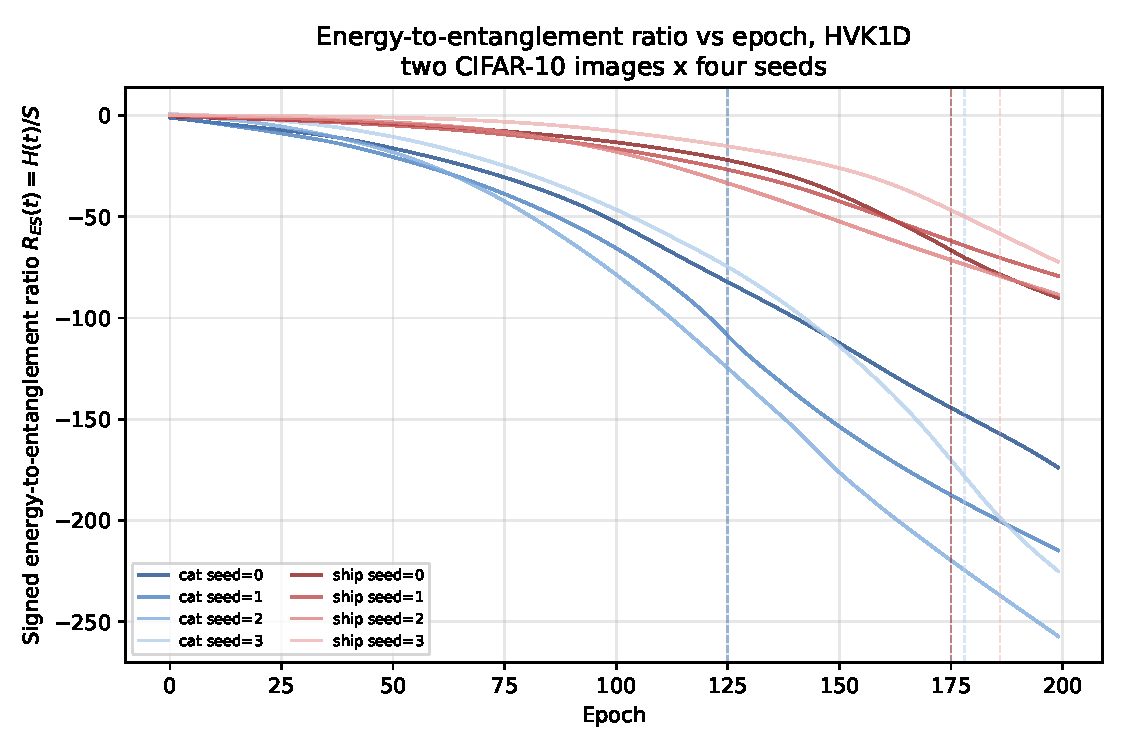
\includegraphics[width=\linewidth]{figures/critical_temperature_traces.pdf}
\caption{Signed energy-to-entanglement ratio $R_{ES}(t)=H(t)/S$ across training, HVK1D, two CIFAR-10 images $\times$ four seeds. The increasingly negative traces reflect the learned signed energy at fixed $S$; they are not temperature or cooling curves.}
\label{fig:critical_temperature}
\end{figure}

\begin{figure}[H]
\centering
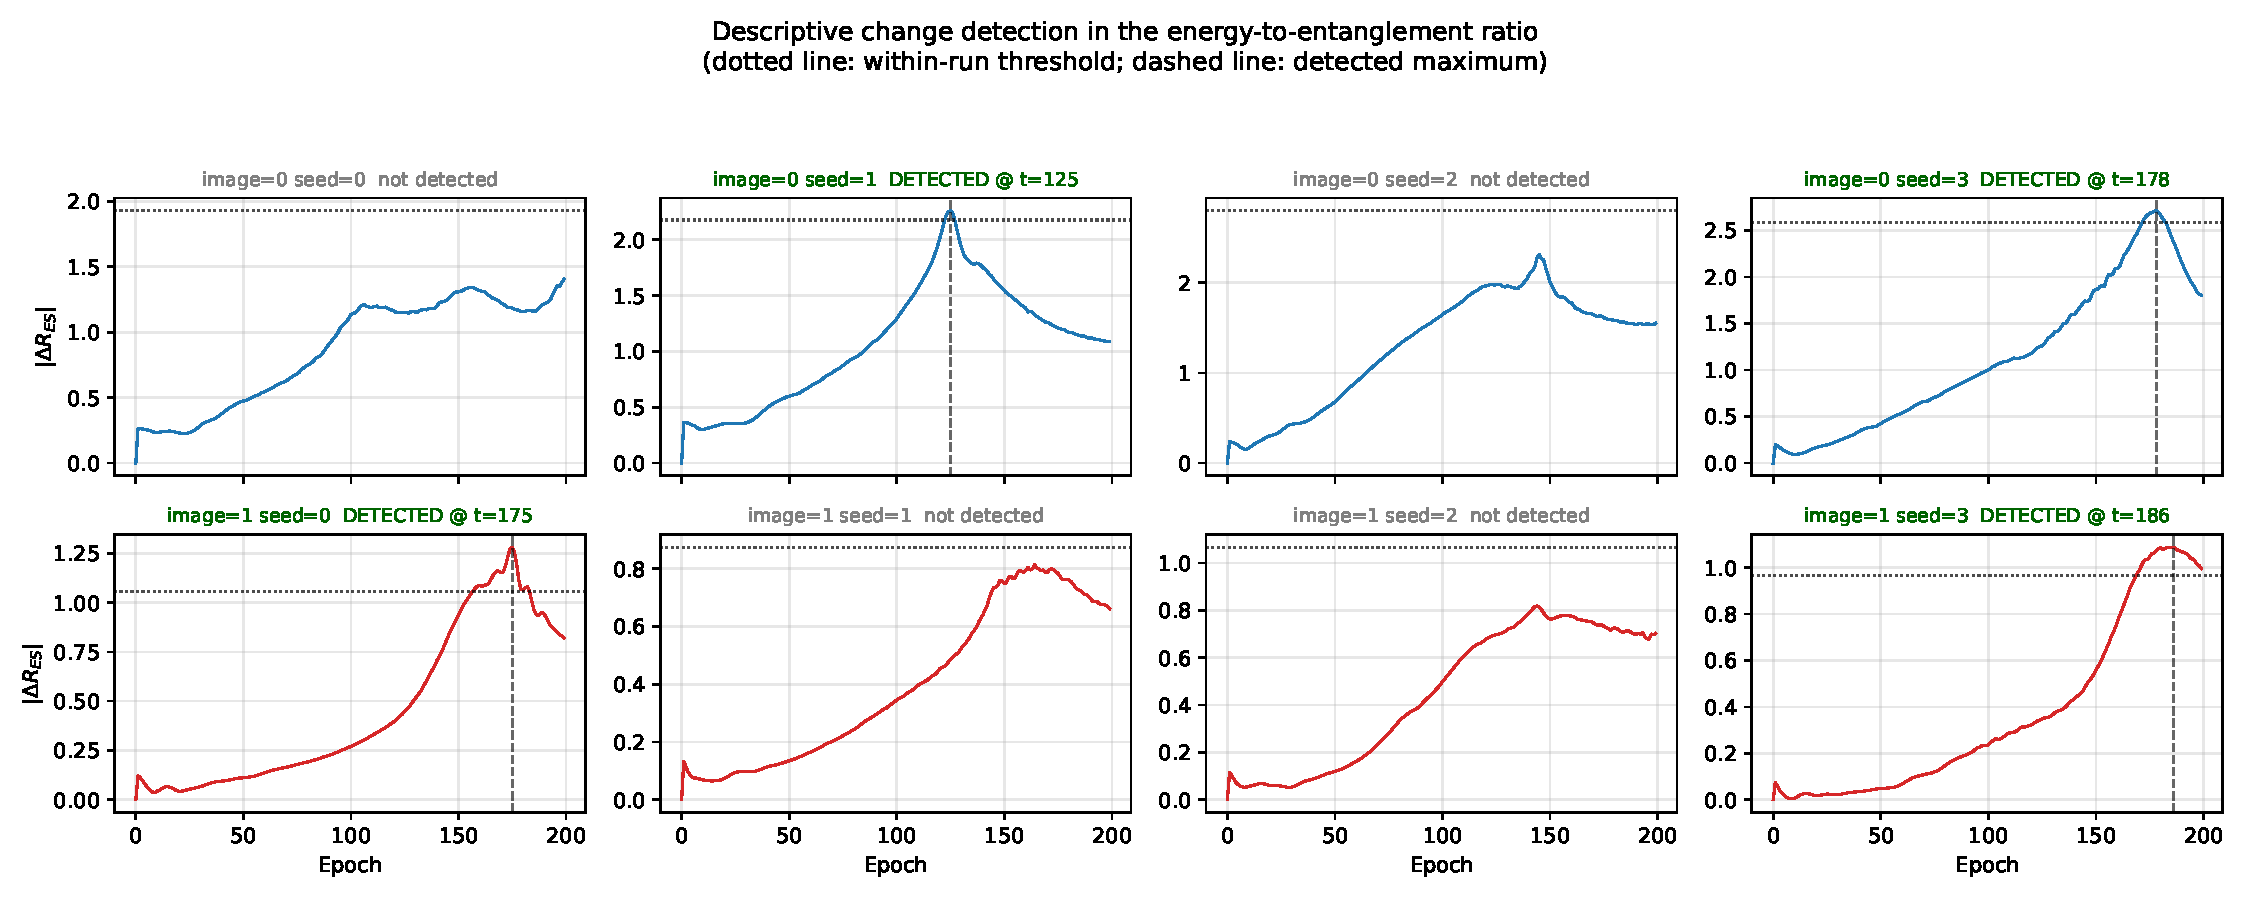
\includegraphics[width=\linewidth]{figures/critical_temperature_susceptibility.pdf}
\caption{Change magnitude $|\Delta R_{ES}(t)|$ vs epoch. The dotted line is the descriptive within-run threshold; a dashed vertical line marks the maximum when it exceeds that threshold.}
\label{fig:critical_temperature_susceptibility}
\end{figure}

All eight $R_{ES}$ traces become more negative as learned signed energy decreases at fixed $S$, and four of eight exceed the descriptive change threshold. Broad peaks occur around epochs 100--180 in every run, but their threshold status depends on within-run scale. The small sample and data-dependent threshold preclude an inferential claim; the result shows only that energy- and magnetization-based summaries can both exhibit nonuniform changes during optimization.

\subsection{Energy-to-Entanglement Ratio, Replayed on Real Hardware}
\label{sec:checkpoint_hardware_energy_entanglement}
Using the same checkpoint-replay methodology as Section~\ref{sec:checkpoint_hardware_finite_size}, we measure $R_{ES}(t)$ itself from real hardware rather than from simulation. The $R_{ES}$ construction requires $N=6$ (Section~\ref{sec:critical_temperature}), so this replay is single-size: we trained fresh HVK1D checkpoints at $N=6$ on the same two images (\textit{Monalisa}, CIFAR-10 \textit{cat}) for 200 real gradient-descent epochs, saved each checkpoint's learned $J_x^{(i)},J_y^{(i)},J_z^{(i)}$ couplings and projected per-qubit angles at the same eight epoch labels, and measured all three Pauli bases needed to reconstruct $\langle X_iX_{i+1}\rangle$, $\langle Y_iY_{i+1}\rangle$, $\langle Z_iZ_{i+1}\rangle$ per bond ($2$ images $\times$ $8$ epoch labels $\times$ $3$ bases $=48$ circuits) on \texttt{ibm\_marrakesh} at $256$, $512$, and $1024$ shots. Hardware-measured bond correlators are combined with each checkpoint's own learned couplings and the fixed, classically-computed bond entropy $S$ to obtain $R_{ES}(t)$; this is a single-patch, single-seed probe, the same limitation noted in Section~\ref{sec:checkpoint_hardware_finite_size}.

As a cross-platform check of the three-basis measurement path, the same 48 circuits were also executed as one 1024-shot job on the IonQ ideal cloud simulator (job identifier retained in the archive). Since this execution used an ideal simulator rather than an IonQ QPU, it supports software-stack portability and estimator reproducibility only.

\begin{figure}[H]
\centering
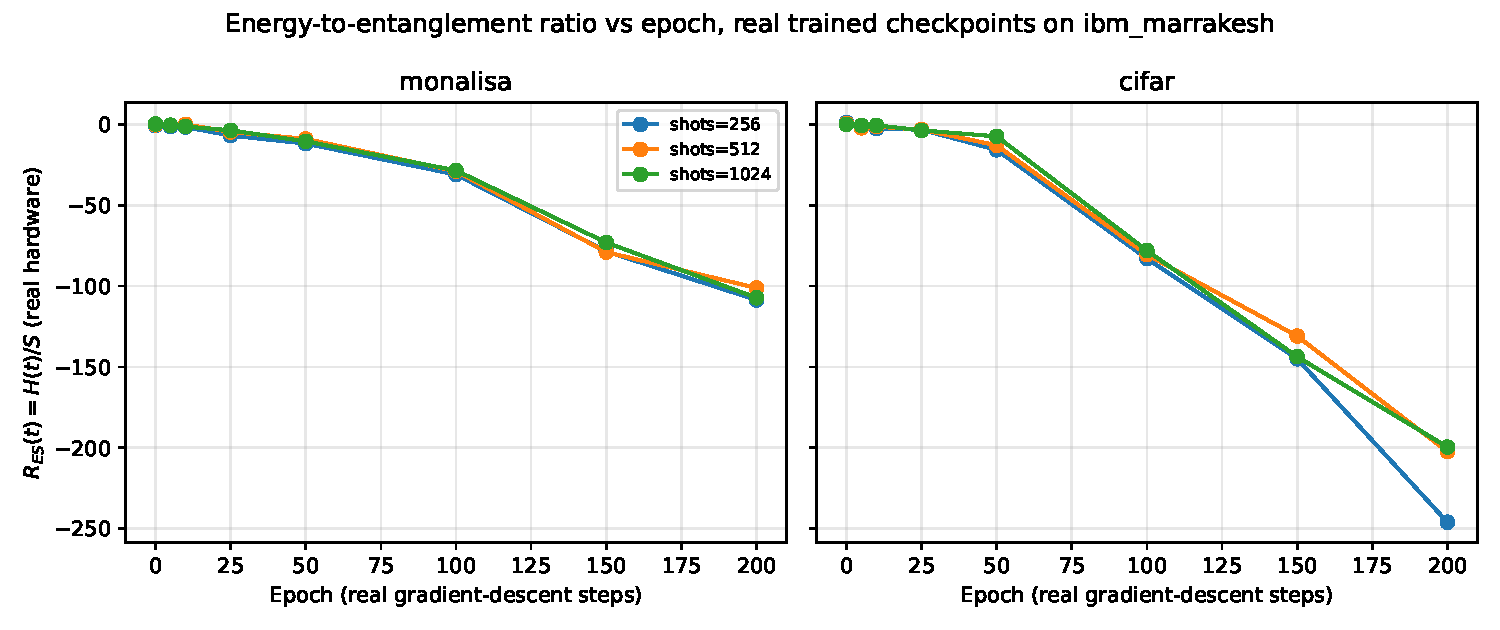
\includegraphics[width=\linewidth]{figures/checkpoint_hardware_energy_entanglement_ratio.pdf}
\caption{$R_{ES}(t)=H(t)/S$ from real trained HVK1D checkpoints ($N=6$), Pauli bond correlators measured on real IBM Quantum hardware (\texttt{ibm\_marrakesh}), one representative patch per image, at three shot budgets.}
\label{fig:checkpoint_hardware_energy_entanglement}
\end{figure}

Figure~\ref{fig:checkpoint_hardware_energy_entanglement} shows the three shot budgets track each other closely for both images, more closely than the order-parameter hardware traces of Figure~\ref{fig:checkpoint_hardware_order_parameter} track across shot budgets --- consistent with $R_{ES}$ summing correlators over multiple bonds and bases, which averages down some of the shot noise visible in the single-qubit order-parameter measurement. As in Section~\ref{sec:checkpoint_hardware_finite_size}, we do not apply the descriptive detection rule to these single-patch traces; the result establishes that hardware-measured bond correlators, combined with a checkpoint's own learned couplings, reproduce a monotonically decreasing $R_{ES}(t)$ consistent in shape with the noiseless-simulator traces of Figure~\ref{fig:critical_temperature}, across three independent shot budgets on real hardware.

\begin{figure}[H]
\centering
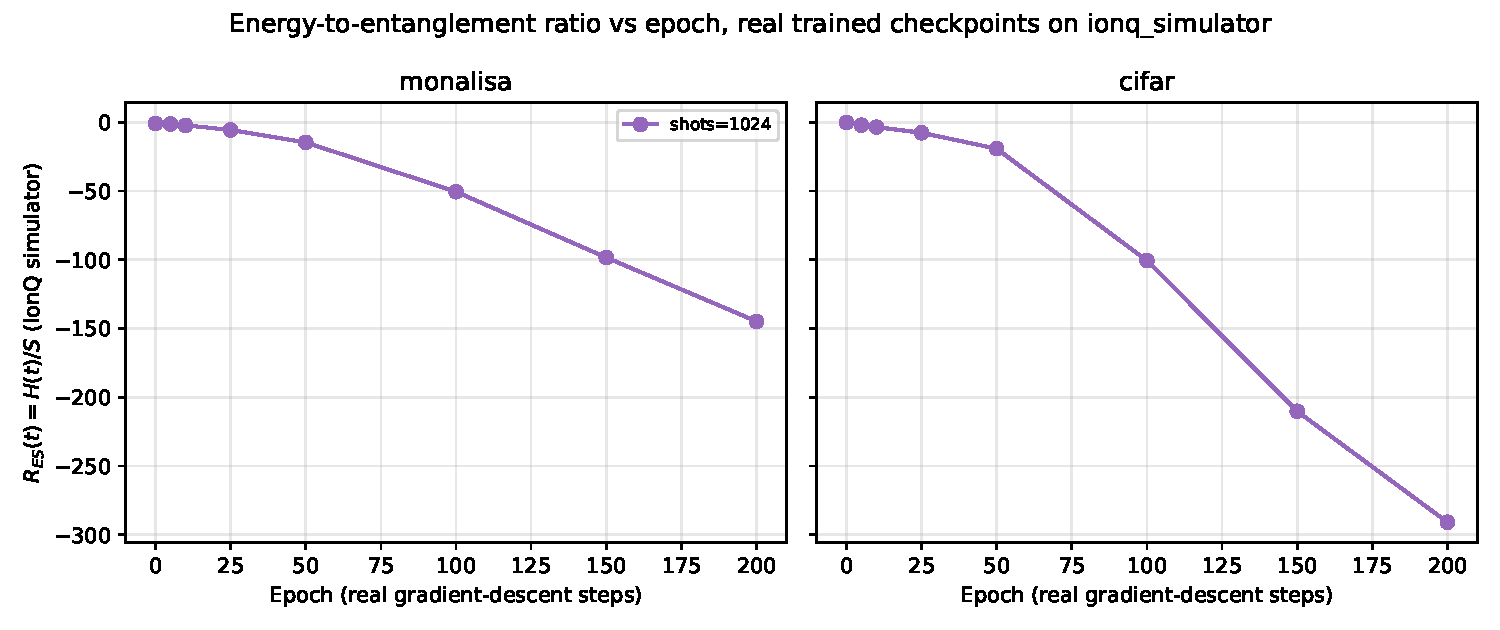
\includegraphics[width=\linewidth]{figures/checkpoint_ionq_energy_entanglement_ratio.pdf}
\caption{$R_{ES}(t)=H(t)/S$ from the same $N=6$ real trained checkpoints as Figure~\ref{fig:checkpoint_hardware_energy_entanglement}, Pauli bond correlators measured instead on the IonQ ideal cloud simulator (1024 shots, the only shot budget submitted for this diagnostic).}
\label{fig:checkpoint_ionq_energy_entanglement}
\end{figure}

Figure~\ref{fig:checkpoint_ionq_energy_entanglement} shows the resulting IonQ traces preserve the same monotonically decreasing shape as the IBM replay above and the noiseless-simulator traces of Figure~\ref{fig:critical_temperature}, for both images. As above, we do not apply the descriptive detection rule of Eq.~\ref{eq:critical_epoch} to these single-patch traces; this is an ideal cloud-simulator portability check, not an IonQ-QPU result.

\section{HVK1D versus HVK2D: A Direct Topology Comparison}
\label{sec:topology_comparison}
The main paper introduces both the HVK1D (6-qubit chain) and HVK2D ($2\times3$ grid) topologies, but until now the only direct comparison was the same-set CIFAR-10 fit of Table~\ref{tab:cifar10}. Here we compare the two topologies directly under matched conditions --- identical qubit count (6, native to both), identical feature width, identical decoder architecture and step budget --- on held-out generalization rather than same-set fitting, on two evidence bases: a fast analytic-surrogate sweep at full statistical scope, and a smaller real-trained-circuit confirmation subset. The two topologies are close in parameter count by construction (HVK1D: 53{,}787; HVK2D: 52{,}755) but not identical, since their circuit structures differ (chain vs. grid connectivity, 27 vs. 19 measured observables); we report this honestly rather than forcing an artificial match.

\subsection{Real-Circuit Confirmation}
\label{sec:topology_real_circuit}
Each topology was trained jointly on 2 CIFAR-10 images (native $32\times32$, overlapping $8\times8$ patches at stride 4, 49 patches/image --- the same convention as Table~\ref{tab:cifar10}) for a reduced 90-step budget across 3 seeds, then evaluated by direct forward pass (no retraining) on 3 further CIFAR-10 images from different classes never seen in training (airplane, frog, automobile) --- a genuine held-out test. The reduced step budget and seed count follow directly from a measured timing calibration on this project's GPU (NVIDIA GTX 1050): at the full 200-step budget used elsewhere in this document, the complete topology comparison at the scope below would cost single-digit hours rather than the tens of minutes actually spent; we report this budget explicitly rather than silently shrinking scope.

\begin{table}[H]
\centering
\caption{Real-trained-circuit topology comparison: held-out reconstruction on 3 unseen CIFAR-10 images (9 image-seed pairs per topology: 3 seeds $\times$ 3 held-out images), 90-step budget.}
\label{tab:topology_real_circuit}
\scriptsize
\begin{tabular}{lcccc}
\toprule
Topology & Params & Held-out PSNR (dB) & Held-out SSIM & Wall time / run (min) \\
\midrule
HVK1D & 53{,}787 & $11.73\pm1.99$ & $0.317\pm0.227$ & $29.6\pm9.0$ \\
HVK2D & 52{,}755 & $11.57\pm1.53$ & $0.304\pm0.188$ & $16.6\pm0.3$ \\
\bottomrule
\end{tabular}
\end{table}

The two topologies give close held-out reconstruction means at this scale. Across the 9 image--seed pairs, the paired HVK1D-minus-HVK2D difference is $0.16$~dB. After aggregating the three image differences within each seed, the seed-bootstrap 95\% CI is $[-0.38,0.46]$~dB and the two-sided Wilcoxon test gives $p=0.50$. The 3-seed, 3-image subset is too small to establish formal equivalence. HVK2D nevertheless completes the same 90-step budget in roughly half the wall-clock time of HVK1D at a comparable parameter count, a measured resource-cost difference. This is consistent with HVK2D's smaller measured observable set (19 vs.\ 27); the corresponding transpiled depth and two-qubit-gate counts are shown in Figure~\ref{fig:ibm_circuit_summary}. At the tested scale, the evidence supports treating topology primarily as a resource-cost choice rather than claiming an accuracy difference.

\subsection{Surrogate Sweep: Full Statistical Scope}
\label{sec:topology_surrogate}
To reach the seed and dataset breadth a held-out comparison needs, we extend the analytic-surrogate held-out framework used above (Tables~\ref{tab:hvk_real_cifar}--\ref{tab:multi_dataset_classification}) with an HVK1D-equivalent feature map. The HVK2D surrogate used there (\texttt{real\_newhvk\_features}) is a closed-form proxy built from six index-pairs of the local-observable block, standing in for the grid circuit's pairwise $ZZ$ correlators. The new HVK1D surrogate is not a relabeled copy: it iterates the chain topology's actual five nearest-neighbor bonds (vs.\ the grid's seven-edge pattern) and adds a second, distinct pair-type term reflecting HVK1D's extra $XX$/$YY$ measurement channels that the 2D grid circuit does not have (it measures only $Z$, $X$, $ZZ$). Both surrogates share the same local/positional input convention, so the comparison is apples-to-apples. We run the full held-out reconstruction and downstream-classification battery (5 seeds, stratified splits) across CIFAR-10, Fashion-MNIST, and PathMNIST.

\begin{table}[H]
\centering
\caption{Surrogate-sweep topology comparison (5 seeds, held-out reconstruction PSNR and downstream classification accuracy), against the strongest classical control (raw-linear) for reference.}
\label{tab:topology_surrogate}
\scriptsize
\begin{tabular}{lccc}
\toprule
Dataset / metric & HVK1D-pair & HVK2D-pair & raw-linear \\
\midrule
CIFAR-10, PSNR (dB) & $19.21\pm2.22$ & $19.28\pm2.25$ & $20.48\pm2.32$ \\
CIFAR-10, accuracy & $0.240\pm0.102$ & $0.260\pm0.102$ & $0.240\pm0.102$ \\
Fashion-MNIST, PSNR (dB) & $17.22\pm1.68$ & $17.24\pm1.69$ & $17.56\pm1.65$ \\
Fashion-MNIST, accuracy & $0.574\pm0.021$ & $0.578\pm0.015$ & $0.654\pm0.020$ \\
PathMNIST, PSNR (dB) & $26.07\pm5.36$ & $26.07\pm5.33$ & $26.60\pm5.57$ \\
PathMNIST, accuracy & $0.560\pm0.046$ & $0.558\pm0.041$ & $0.596\pm0.041$ \\
\bottomrule
\end{tabular}
\end{table}

\begin{figure*}[t]
\centering
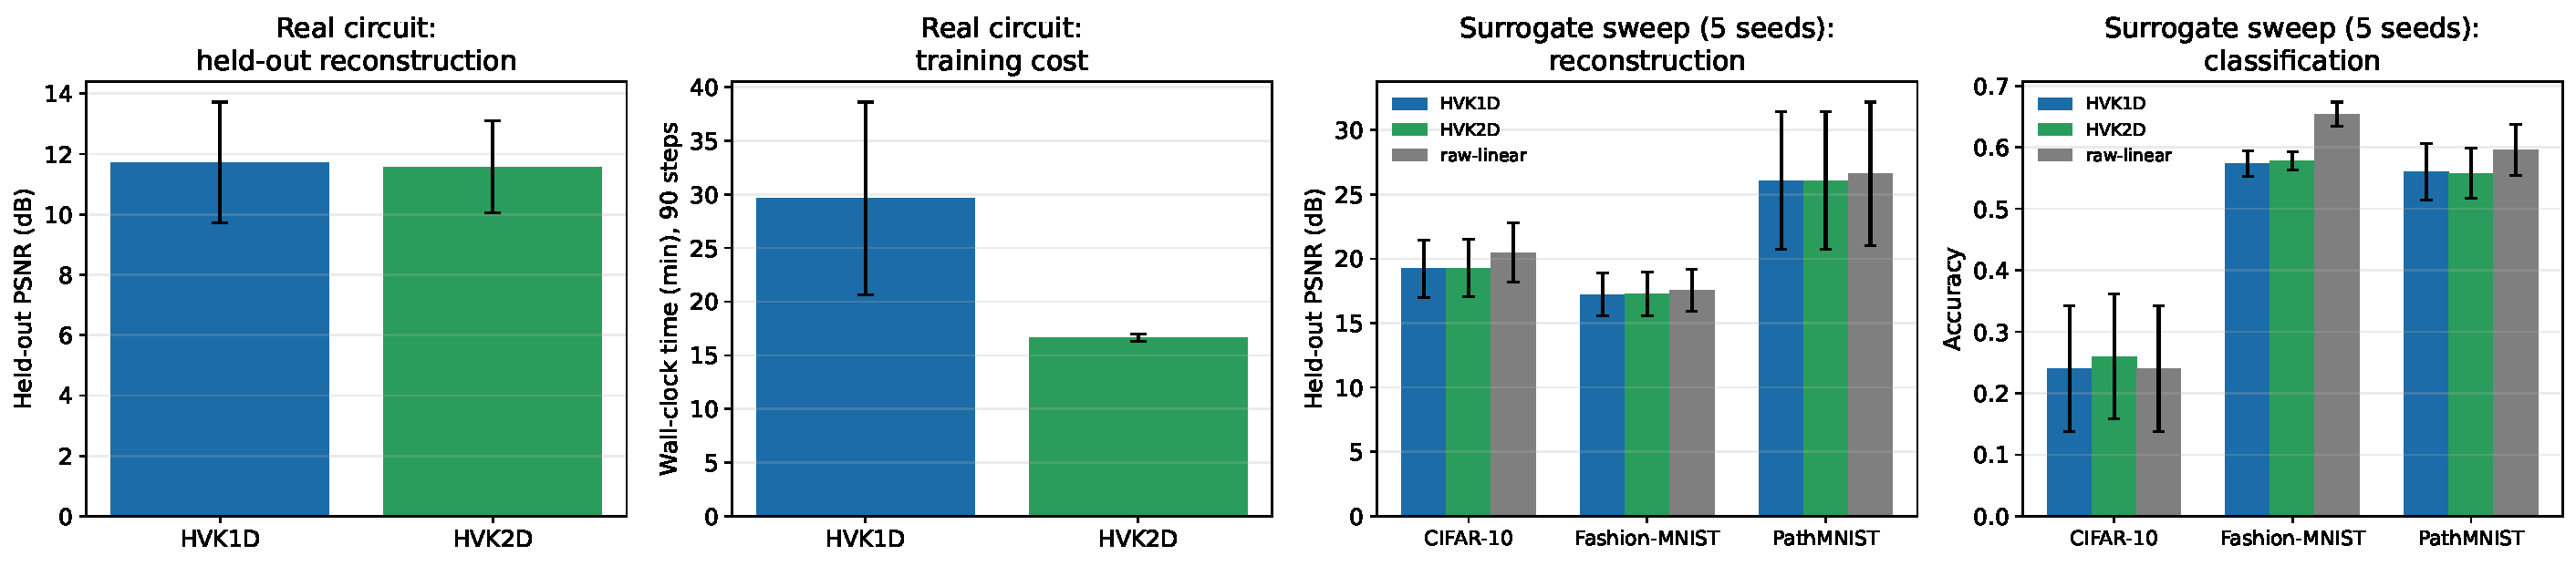
\includegraphics[width=0.95\textwidth]{figures/topology_comparison_summary.pdf}
\caption{HVK1D vs.\ HVK2D across both evidence bases. Left two panels: real-circuit held-out PSNR and per-run wall-clock time (90-step budget, 3 seeds, error bars = std). Right two panels: surrogate-sweep held-out reconstruction PSNR and classification accuracy across three datasets (5 seeds), both topologies plotted against the strongest classical control (raw-linear).}
\label{fig:topology_comparison_summary}
\end{figure*}

The broader surrogate sweep reproduces the real-circuit pattern: HVK1D-pair and HVK2D-pair track each other closely on every dataset and metric (PSNR differs by at most $0.07$~dB, accuracy by at most $2$ percentage points), and both sit slightly below the raw-linear control. For inference, held-out image differences are first averaged within each split seed so that images sharing a fitted readout are not treated as independent replicates. The seed-level HVK1D-minus-HVK2D PSNR differences are $-0.070$~dB on CIFAR-10 (bootstrap 95\% CI $[-0.151,0.024]$, Wilcoxon $p=0.3125$), $-0.021$~dB on Fashion-MNIST (CI $[-0.033,-0.006]$, $p=0.125$), and $0.003$~dB on PathMNIST (CI $[-0.012,0.015]$, $p=0.625$), all at $n=5$ seeds. The Fashion-MNIST percentile interval excludes zero, but the discrete seed-level signed-rank test does not resolve the difference; we therefore describe it as numerically small rather than statistically established. Neither topology shows a general reconstruction/classification advantage over simple classical baselines, and the evidence supports treating topology as a resource-cost choice at the tested scale. Section~\ref{sec:restricted_ablation}'s restricted, leakage-audited diagnostic remains the setting where entanglement structure matters within the tested feature/readout class.

\section{Held-Out Output-Level \texorpdfstring{$D_4$}{D4} Symmetry Evaluation}
\label{sec:d4_symmetry_experiment}
The main paper's $D_4$-equivariance claim (pooled HVK2D observable map, equivariance error $9.57\times10^{-17}$) was previously demonstrated at feature-grid level on 1,000 cached CIFAR-10 images, giving 7,000 image--nonidentity-transform evaluations. That large numerical check did not use a fitted readout, a held-out reconstruction protocol, or a classical baseline sharing the same pooling construction, and therefore did not measure what equivariance costs or buys at the output level. This section closes those gaps with a held-out, multi-seed (5 seeds, 20 train / 10 held-out images per seed, disjoint CIFAR-10 splits) experiment across five modes: the provably-equivariant \emph{D4-pooled-HVK2D} map; a new \emph{D4-pooled-classical} baseline applying the identical Reynolds-averaging construction (group-averaging the feature map over the eight $D_4$ transforms) to the purely classical \emph{local-raw} feature map instead of the HVK2D-surrogate one, so the comparison is architecture-matched rather than quantum-vs-nothing; the non-symmetric \emph{HVK2D-positional} control; an \emph{ordinary-augmentation} baseline (\emph{HVK2D-augmented}: the same non-pooled feature map, but with a ridge readout trained on all eight $D_4$-transformed copies of every training image, instead of architectural pooling); and the non-symmetric classical \emph{local-raw} control. For every mode we measure both \emph{feature-equivariance error} (as before) and, new here, \emph{output consistency}: for each held-out image we predict a reconstruction from every one of its 8 $D_4$-transformed copies, rotate/reflect each prediction back to canonical orientation, and measure the pairwise mean-squared disagreement between the 8 canonicalized predictions, together with reconstruction accuracy (PSNR) against ground truth.

\begin{table}[H]
\centering
\caption{Held-out output-level $D_4$ symmetry evaluation (5 seeds, 10 held-out images/seed). Feature-equivariance error and output-consistency MSE are reported at $\pm$std over seeds; both span many orders of magnitude between pooled and non-pooled modes.}
\label{tab:d4_symmetry_experiment}
\scriptsize
\begin{tabular}{lccc}
\toprule
Mode & Equivariance error & Output consistency (MSE) & Accuracy PSNR (dB) \\
\midrule
D4-pooled (HVK2D) & $(9.47\pm0.25)\times10^{-17}$ & $(3.19\pm1.66)\times10^{-21}$ & $14.97\pm0.53$ \\
D4-pooled (classical) & $(8.94\pm0.22)\times10^{-17}$ & $(1.37\pm0.96)\times10^{-23}$ & $15.12\pm0.52$ \\
HVK2D (non-symmetric) & $0.8163\pm0.0070$ & $0.01149\pm0.00213$ & $15.12\pm0.59$ \\
HVK2D (ordinary aug.) & $0.8163\pm0.0070$ & $0.01055\pm0.00226$ & $15.30\pm0.56$ \\
local-raw (classical) & $0.8380\pm0.0067$ & $0.01202\pm0.00245$ & $15.16\pm0.68$ \\
\bottomrule
\end{tabular}
\end{table}

\begin{figure*}[t]
\centering
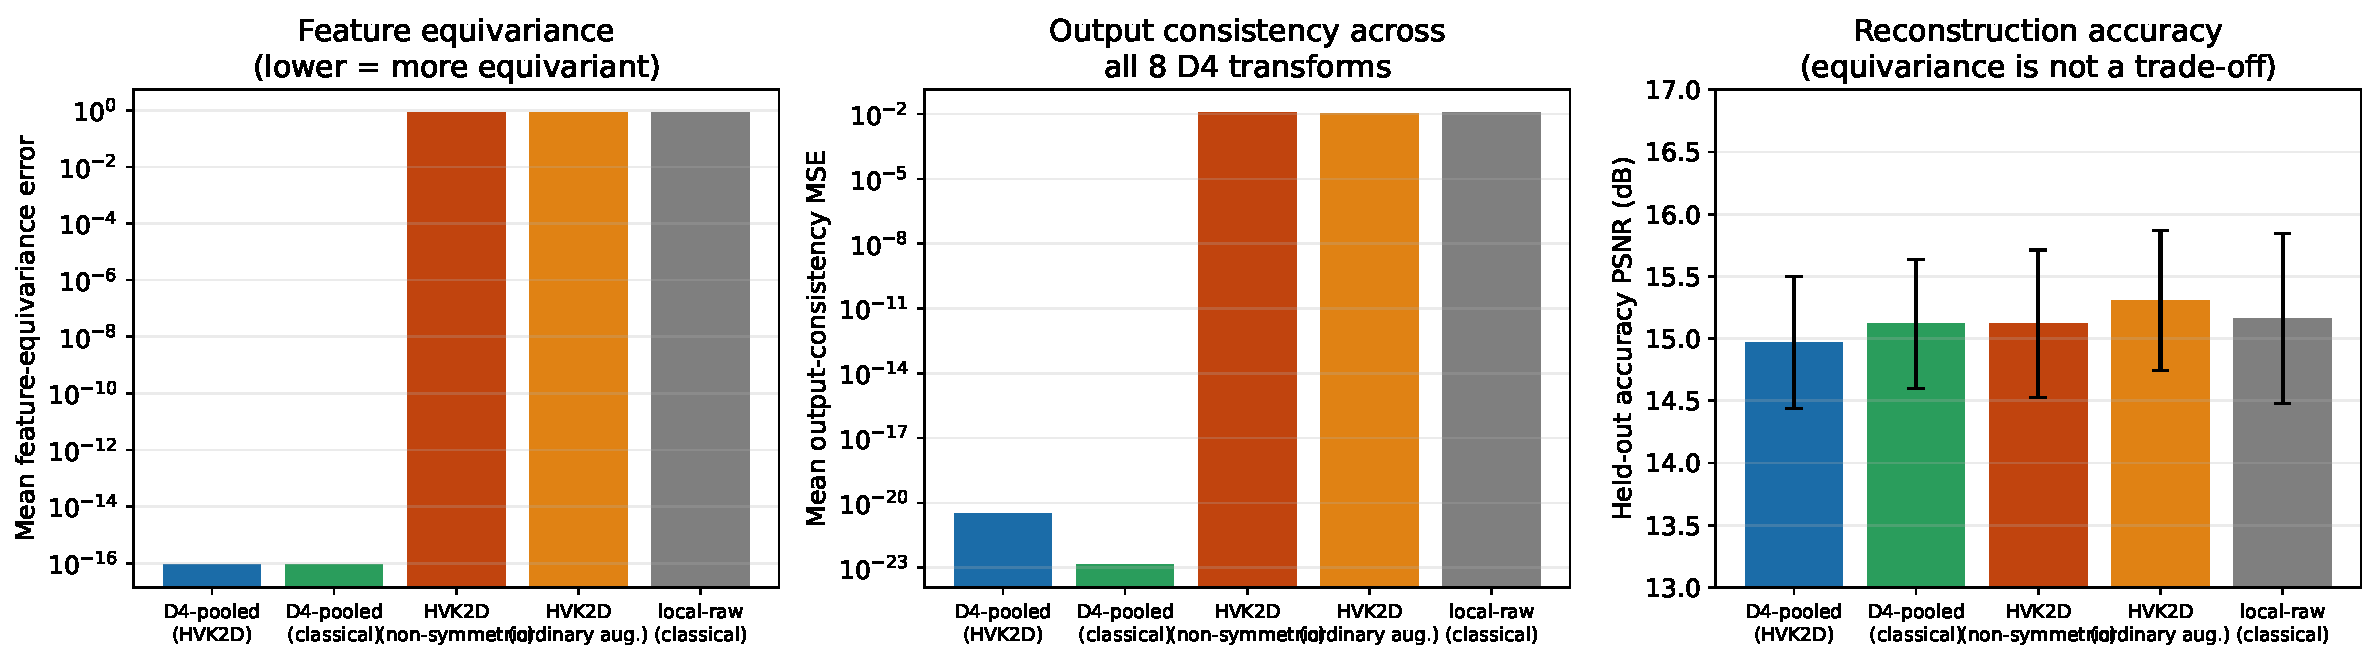
\includegraphics[width=0.95\textwidth]{figures/d4_symmetry_experiment_summary.pdf}
\caption{Held-out output-level $D_4$ symmetry evaluation, 5 seeds. Left: feature-equivariance error (log scale) --- both pooled modes sit at floating-point precision, roughly 16 orders of magnitude below every non-pooled control. Center: output-consistency MSE across all 8 $D_4$ transforms (log scale) --- the same separation persists at the reconstruction-output level, not just the feature level. Right: held-out accuracy PSNR (linear scale, error bars = std) --- the five mean values are close relative to their between-seed variation; no formal equivalence claim is made.}
\label{fig:d4_symmetry_experiment_summary}
\end{figure*}

Four findings follow. First, the Reynolds-averaging construction that gives HVK2D its provable equivariance is not specific to the quantum-surrogate feature map: applying the identical pooling operation to a purely classical local-observable map produces the same floating-point-precision equivariance ($8.94\times10^{-17}$ vs.\ $9.47\times10^{-17}$), confirming the guarantee is a property of the group-averaging construction itself, not of anything intrinsically quantum. Second, the separation between pooled and non-pooled modes is not an artifact of measuring features in isolation: it persists essentially unchanged at reconstruction output (output-consistency MSE $\sim10^{-21}$--$10^{-23}$ for pooled modes vs.\ $\sim0.010$--$0.012$ for non-pooled controls). Third, ordinary augmentation cannot change feature-equivariance error, but it reduces output-consistency MSE by roughly $8\%$ ($0.01055$ vs.\ $0.01149$). Fourth, exact pooling has a small accuracy trade-off relative to ordinary augmentation: pooled HVK2D is lower by $0.336$~dB on average across the five paired seeds (seed-bootstrap 95\% CI $[-0.441,-0.231]$~dB; two-sided Wilcoxon $p=0.0625$, the smallest attainable nonzero two-sided value at $n=5$). The symmetry guarantee is decisive, while the available sample supports a modest rather than zero accuracy cost.

\subsection{Real-Circuit Confirmation}
\label{sec:d4_real_circuit}
Everything above is measured on the closed-form analytic surrogate. This subsection repeats the pooled-vs-non-pooled equivariance and output-consistency comparison on the \emph{actual trained quantum circuit} --- the same four already-trained HVK2D checkpoints used for the main paper's real IBM-hardware pilot (\textit{cat}, \textit{ship/hydrofoil}, \textit{ship/sea boat}, \textit{airplane}), replayed with no retraining. For each image we run the trained model's real PennyLane forward pass (exact statevector simulation of the trained weights, not the surrogate formula) on all eight $D_4$-transformed copies of the full image, and compute the same feature-equivariance error and output-consistency MSE as above, both without pooling and with the identical Reynolds-averaging construction applied to the real circuit's own output grid.

\begin{table}[H]
\centering
\caption{Real-trained-circuit $D_4$ confirmation: exact PennyLane forward pass on four already-trained HVK2D hardware-pilot checkpoints, no retraining.}
\label{tab:d4_real_circuit}
\scriptsize
\begin{tabular}{lccc}
\toprule
Image & Mode & Equivariance error & Output consistency (MSE) \\
\midrule
cat & non-pooled & $0.0760$ & $0.01869$ \\
cat & D4-pooled & $5.50\times10^{-8}$ & $9.78\times10^{-16}$ \\
ship (hydrofoil) & non-pooled & $0.3905$ & $0.06437$ \\
ship (hydrofoil) & D4-pooled & $5.25\times10^{-8}$ & $1.83\times10^{-15}$ \\
ship (sea boat) & non-pooled & $0.4054$ & $0.05451$ \\
ship (sea boat) & D4-pooled & $5.65\times10^{-8}$ & $1.24\times10^{-15}$ \\
airplane & non-pooled & $0.2387$ & $0.03662$ \\
airplane & D4-pooled & $5.16\times10^{-8}$ & $1.80\times10^{-15}$ \\
\midrule
Mean & non-pooled & $0.2777$ & $0.04355$ \\
Mean & D4-pooled & $5.39\times10^{-8}$ & $1.46\times10^{-15}$ \\
\bottomrule
\end{tabular}
\end{table}

The real-circuit result confirms the surrogate's finding directly: pooling collapses the equivariance error from $\mathcal{O}(10^{-1})$ to $\mathcal{O}(10^{-8})$ and output-consistency MSE from $\mathcal{O}(10^{-2})$ to $\mathcal{O}(10^{-15})$, an 8--13 order-of-magnitude gap on every one of the four images, with no exceptions. The pooled real circuit's residual error ($\sim\!5\times10^{-8}$) is larger than the surrogate's floating-point-precision result ($\sim\!10^{-17}$) because the real circuit involves a full statevector simulation of the trained gates plus a fresh per-transform feature-standardization step, both of which accumulate ordinary floating-point noise that the closed-form surrogate formula does not --- the pooled result is exact up to numerical precision, not exact to the same sixteen digits as a symbolic identity, which is the expected and unremarkable difference between an analytic proxy and an actual simulated circuit.

\section{Exact Circuit and Hamiltonian Definitions}
\label{sec:supp_exact_circuits}
For a one-dimensional chain of $n_{\text{bonds}}$ bonds indexed by $i$ and sites $(i,i+1)$, the anisotropic Heisenberg Hamiltonian is
\begin{align}
H_{\text{Heis}}=\sum_{i=0}^{n_{\text{bonds}}-1}\Bigl(
J_x^{(i)}X_iX_{i+1}+J_y^{(i)}Y_iY_{i+1}\nonumber\\
{}+J_z^{(i)}Z_iZ_{i+1}\Bigr).
\end{align}
Here $X,Y,Z$ are Pauli operators and $J_\alpha^{(i)}$ are bond-resolved couplings. HVK1D fixes six sites and treats the 15 coefficients on its five bonds as learnable parameters initialized independently from a zero-mean Gaussian with standard deviation $0.1$. Given patch $n$'s measured observables, its energy diagnostic is
\begin{equation}
\mathcal{E}_n(\theta,J) = \sum_{i=0}^{4}\sum_{\alpha\in\{x,y,z\}} J_\alpha^{(i)}\langle\sigma_\alpha^{(i)}\sigma_\alpha^{(i+1)}\rangle_n.
\end{equation}
HVK2D instead uses the seven edges $\mathcal{G}_{2D}$ of its $2\times3$ circuit graph and the implemented grid-Ising diagnostic $\mathcal{E}^{2D}_n=\sum_{(u,v)\in\mathcal{G}_{2D}}j_{uv}\langle Z_uZ_v\rangle_n$. Thus ``Hamiltonian diagnostic'' refers to the full $XX/YY/ZZ$ chain energy for HVK1D and the learned $ZZ$ graph energy for HVK2D. In either case, the patch-averaged term is $\mathcal{L}_{\text{energy}}=\frac{1}{N}\sum_n \mathcal{E}_n$, and the total objective is
\begin{align}
\mathcal{L}_{\text{total}}&=\mathcal{L}_{\text{rec}}
+\lambda\,\mathcal{L}_{\text{energy}},\\
\mathcal{L}_{\text{rec}}&=\frac{1}{N}\sum_{n=1}^{N}
\bigl\|D(o_n,e_n)-P_n\bigr\|_F^2.
\end{align}
with $D$ the classical decoder and $P_n$ the ground-truth patch.

\begin{sloppypar}
Per-patch coordinates $(r_i,c_j)$ are mapped to Fourier features $e_{4k}=\sin(\omega_k\pi r_i)$, $e_{4k+1}=\cos(\omega_k\pi r_i)$, $e_{4k+2}=\sin(\omega_k\pi c_j)$, and $e_{4k+3}=\cos(\omega_k\pi c_j)$ \cite{Xu2021}. HVK1D uses $k\in\{0,1\}$ (8-D), whereas the native-resolution HVK2D implementation uses one frequency (4-D); a learned linear map projects either vector to six $R_Y$ angles. Both six-qubit circuits first apply $U_{\text{enc}}(x_n)=\bigotimes_{i=0}^{5}R_X(x_n^{(i)})$ and $U_{\text{pos}}=\bigotimes_{i=0}^{5}R_Y(\theta_{\text{position}}^{(i)})$. Each of two HVK1D layers then applies per-qubit $\mathrm{Rot}$ gates followed by the strongly-entangling CNOT ring. Each HVK2D layer applies CNOTs over the four horizontal and three vertical grid edges followed by per-qubit $\mathrm{Rot}$ gates, matching the executed source and hardware-replay circuits.

HVK1D returns local $Z/X$ measurements and the three nearest-neighbor pair sectors $ZZ/XX/YY$ (27 values); HVK2D returns local $Z/X$ measurements and grid-edge $ZZ$ correlations (19 values). Positional rotations and fixed graph connectivity distinguish circuit sites, so neither unpooled map is asserted to be permutation- or $D_4$-equivariant. The $D_4$ action in the main paper is instead the explicit permutation action on the $4\times4$ patch grid, and equivariance follows only after the stated Reynolds average over its eight transformations.
\end{sloppypar}

\section{Hardware Pilot Methodology}
\label{sec:hardware_methodology}
The main paper reports a real IBM Quantum hardware reconstruction pilot (five images: \textit{Monalisa} and four CIFAR-10 images, each optimized per-image, hardware PSNR $25.90$--$31.52$~dB against $36.56$--$46.79$~dB in noiseless simulation). This section gives the complete methodology.

\subsection{Reused Checkpoints}
No model was retrained for this pilot. Two pre-existing artifacts were reused directly. The first was the ``shared VQC baseline'' Monalisa checkpoint under
\begin{quote}
\small\path{main2/newHVK/results/ablation_study/legacy_hvk_controls/eval_controls/}\newline\path{shared-baseline-seed-42/}.
\end{quote}
This is the run underlying the ``Legacy baseline, signed energy'' row of Table~\ref{tab:hamiltonian_controls} ($32.24$~dB simulator PSNR). The second set comprised four fresh HVK2D checkpoints trained for 200 steps with Adam ($\eta=0.004$) on an NVIDIA GTX~1050. Each checkpoint corresponds to one native-resolution $32\times32$ CIFAR-10 image optimized directly on its own target, following the same per-image protocol as \textit{Monalisa} rather than the held-out suite of Section~\ref{sec:holdout_headline}. Non-overlapping $8\times8$ patches give 16 patches per image, matching the Monalisa pilot's patch count and keeping the hardware circuit budget predictable.

\subsection{Circuit Reconstruction}
The trained HVK1D forward pass applies, per patch: $R_X$ angle embedding, $R_Y$ positional modulation, then two \texttt{StronglyEntanglingLayers} (per-wire $R_Z$-$R_Y$-$R_Z$ rotations with a CNOT ring whose range increments by layer). We rebuilt this gate-for-gate in Qiskit. Because the trained circuit measures $Z$, $X$, $ZZ$, $XX$, and $YY$ (27 observables), and pairwise correlators are recoverable as joint parities of the \emph{same} all-$Z$/all-$X$/all-$Y$ basis measurements that already give the single-qubit marginals, only three measurement circuits per patch are needed. For 16 Monalisa patches this is $16\times3=48$ circuits. The HVK2D grid circuit is simpler (two layers of fixed grid-edge CNOTs then per-qubit rotations) and measures only $Z$, $X$, $ZZ$ (19 observables, no $XX$/$YY$), so only two measurement circuits per patch are needed: for four CIFAR images at 16 patches each, $4\times16\times2=128$ circuits.

\begin{figure}[H]
\centering
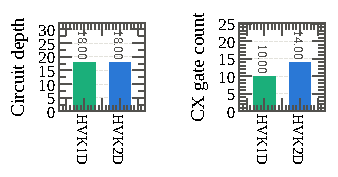
\includegraphics[width=0.75\linewidth]{figures/ibm_circuit_summary.pdf}
\caption{Transpiled circuit resource comparison between the HVK1D (\textit{Monalisa}) and HVK2D (CIFAR) per-patch circuits at \texttt{optimization\_level=1} on \texttt{ibm\_fez}: circuit depth (left) and CX-gate count (right). Both circuits have depth 18 and use 10--14 CX gates. These resource counts document the executed circuits; they do not by themselves attribute the observed hardware--simulator PSNR gap to a particular noise source.}
\label{fig:ibm_circuit_summary}
\end{figure}

\subsection{Local Validation Before Any Hardware Submission}
Every circuit was validated against the cached, training-time observable vectors via an exact Qiskit statevector simulation, \emph{before} any job was submitted to real hardware.

\begin{table}[H]
\centering
\caption{Local validation: Qiskit statevector reconstruction vs.\ cached PennyLane training-time observables.}
\begin{tabular}{lcc}
\toprule
Checkpoint & Patches validated & Max abs.\ error \\
\midrule
Monalisa (HVK1D) & 16 & $7.89\times10^{-4}$ \\
CIFAR cat (HVK2D) & 16 & $9.42\times10^{-6}$ \\
CIFAR ship, hydrofoil (HVK2D) & 16 & $7.76\times10^{-6}$ \\
CIFAR ship, sea boat (HVK2D) & 16 & $7.89\times10^{-6}$ \\
CIFAR airplane (HVK2D) & 16 & $7.14\times10^{-6}$ \\
\bottomrule
\end{tabular}
\end{table}

All translation discrepancies are small relative to the observable perturbations induced by finite-shot device execution: across the five checkpoints, the hardware--statevector mean absolute observable deviation is $0.096$--$0.125$ (maximum $0.218$--$0.340$), versus a maximum translation discrepancy of $7.89\times10^{-4}$ for Monalisa and $9.42\times10^{-6}$ for CIFAR. They therefore rule out a gate-translation mismatch of the measured magnitude as the primary explanation for the hardware--simulator PSNR gap. This pilot does not separate sampling noise, gate/readout errors, drift, and transpilation effects.

\subsection{IBM Quantum Account, Backend, and Job Identifiers}
Jobs were submitted via \texttt{qiskit-ibm-runtime} (channel \texttt{ibm\_quantum\_platform}) under a free/open-plan instance. Both pilots ran on \texttt{ibm\_fez}, a 156-qubit Heron-class processor. Transpilation used \texttt{optimization\_level=1}; each job used \texttt{SamplerV2} with 256 shots per circuit.

\begin{table}[H]
\centering
\caption{IBM Quantum job identifiers (backend: \texttt{ibm\_fez}, 256 shots/circuit).}
\scriptsize
\begin{tabular}{llcc}
\toprule
Image & Job ID & Circuits & Bases \\
\midrule
Monalisa & \texttt{d9ecu34inv1c73aq3qt0} & 48 & Z, X, Y \\
CIFAR cat & \texttt{d9edfo2neu4c739ob2ig} & 32 & Z, X \\
CIFAR ship (hydrofoil) & \texttt{d9edg5cjeosc73filhng} & 32 & Z, X \\
CIFAR ship (sea boat) & \texttt{d9edgakjeosc73filhug} & 32 & Z, X \\
CIFAR airplane & \texttt{d9edgdphtsac739e4kdg} & 32 & Z, X \\
\bottomrule
\end{tabular}
\end{table}

Total: 176 circuits across 5 jobs. Quota consumption, read from \texttt{QiskitRuntimeService.}\allowbreak\texttt{usage()} immediately before and after the pilot, changed from $19$ to $35$ seconds against a $600$-second monthly free-plan allowance. Thus the account meter indicated 16 seconds of billed quantum-processor time and 565 seconds remaining afterward, at an observed rate of $\approx\!0.09$--$0.13$~s/circuit. The readings were recorded contemporaneously, but the raw service-response object was not serialized; unlike the job identifiers and reconstruction outputs, this quota figure is therefore an execution-log record rather than a repository-recomputable artifact.

\subsection{IonQ Ideal Cloud-Simulator Replay}
The main paper's cross-platform check used IonQ Quantum Cloud's ideal simulator through the Qiskit provider, with no device-noise model. It therefore tests circuit translation, submission, count retrieval, bit-order handling, and estimator reproducibility, but is not an IonQ-QPU experiment. Each order-parameter job contained 48 circuits: two images (\textit{Monalisa}, CIFAR-10 \textit{cat}), three widths $N\in\{4,6,8\}$, and eight checkpoint epochs. Counts were reduced with the same $M_z$, nearest-neighbor $ZZ$, and proxy-loss estimators as the IBM replay.

\begin{table}[H]
\centering
\caption{IonQ ideal cloud-simulator order-parameter replay. Deviations use the independently sampled 1024-shot IonQ trace at matched image, width, and epoch as the reference.}
\scriptsize
\resizebox{\linewidth}{!}{%
\begin{tabular}{lcccl}
\toprule
Shots & Circuits & Mean $|{\Delta M_z}|$ & Max $|{\Delta M_z}|$ & Job ID \\
\midrule
256  & 48 & 0.0257 & 0.0902 & \texttt{019f903b-62c0-74db-adec-a33847ae8a1c} \\
512  & 48 & 0.0213 & 0.0581 & \texttt{019f903d-09d4-7548-87f1-2a55185ee9b5} \\
1024 & 48 & Reference & Reference & \texttt{019f903e-cac2-708f-911f-67b2b6d7471c} \\
\bottomrule
\end{tabular}
}
\end{table}

A second IonQ ideal-simulator job (\texttt{019f9046-7ba6-7320-9766-552d88d490bf}) executed the 48 three-basis circuits required for the energy-to-entanglement ratio at 1024 shots. It reproduced the decreasing $R_{ES}(t)$ trajectory shape for both images. Because these are ideal finite-shot simulations, the numerical differences above describe sampling and cross-stack agreement only; they do not support claims about IonQ hardware noise, QPU quality, or comparative hardware performance.

\subsection{Bond-Dimension Checkpoint Replays}
\label{sec:supp_bond_dimension_hardware}
The main paper's bond-dimension replay fixes $N=6$, varies the MPS bond dimension over $\chi\in\{1,2,4,8\}$, and uses two images, one representative patch, one training seed, and eight checkpoint epochs. At each shot budget, the order-parameter job therefore contains $2\times4\times8=64$ circuits. We executed the same circuit set on real IBM hardware (\texttt{ibm\_marrakesh}) and the IonQ ideal cloud simulator at 256, 512, and 1024 shots. This is an execution and portability check across trained checkpoints; one seed per $\chi$ cannot confirm the simulator study's cross-seed variance pattern.

\begin{figure}[H]
\centering
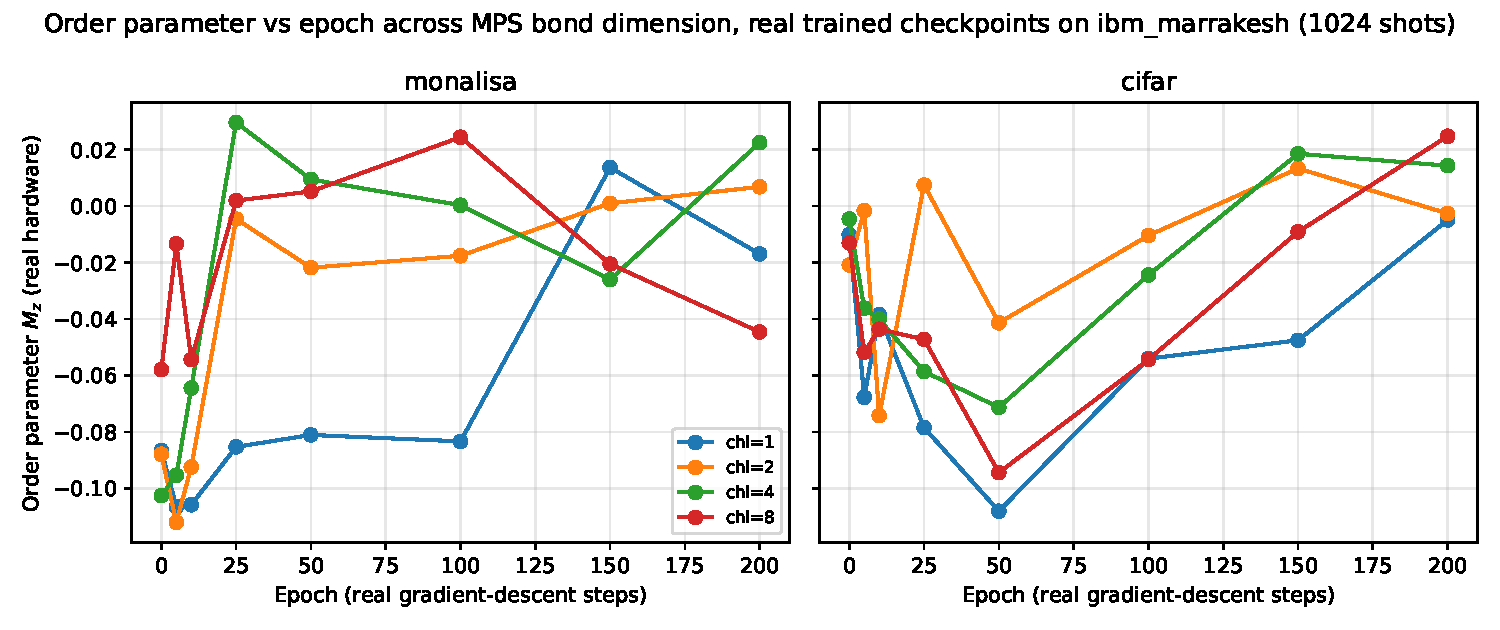
\includegraphics[width=0.9\linewidth]{figures/checkpoint_hardware_bond_dimension_order_parameter.pdf}
\caption{Bond-dimension checkpoint replay at 1024 shots on real IBM Quantum hardware. The plotted $M_z(t)$ traces use one representative patch and seed per image and $\chi$.}
\label{fig:supp_checkpoint_hardware_bond_dimension}
\end{figure}

\begin{table}[H]
\centering
\caption{Bond-dimension order-parameter replay jobs. Each job contains 64 circuits.}
\scriptsize
\resizebox{\linewidth}{!}{%
\begin{tabular}{llll}
\toprule
Platform & Backend & Shots & Job ID \\
\midrule
IBM hardware & \texttt{ibm\_marrakesh} & 256 & \texttt{d9hqu0jsbqfc73eqgr80} \\
IBM hardware & \texttt{ibm\_marrakesh} & 512 & \texttt{d9hr3d8gk0ls73f3elsg} \\
IBM hardware & \texttt{ibm\_marrakesh} & 1024 & \texttt{d9hr43l0k0jc738il8ug} \\
IonQ ideal simulator & \texttt{ionq\_simulator} & 256 & \texttt{019f9571-21d0-7339-9111-d31a308440a1} \\
IonQ ideal simulator & \texttt{ionq\_simulator} & 512 & \texttt{019f9573-1ed9-768c-9768-465fe75a409b} \\
IonQ ideal simulator & \texttt{ionq\_simulator} & 1024 & \texttt{019f9574-a981-71dd-94b0-9d8fb8968f49} \\
\bottomrule
\end{tabular}
}
\end{table}

\begin{figure}[H]
\centering
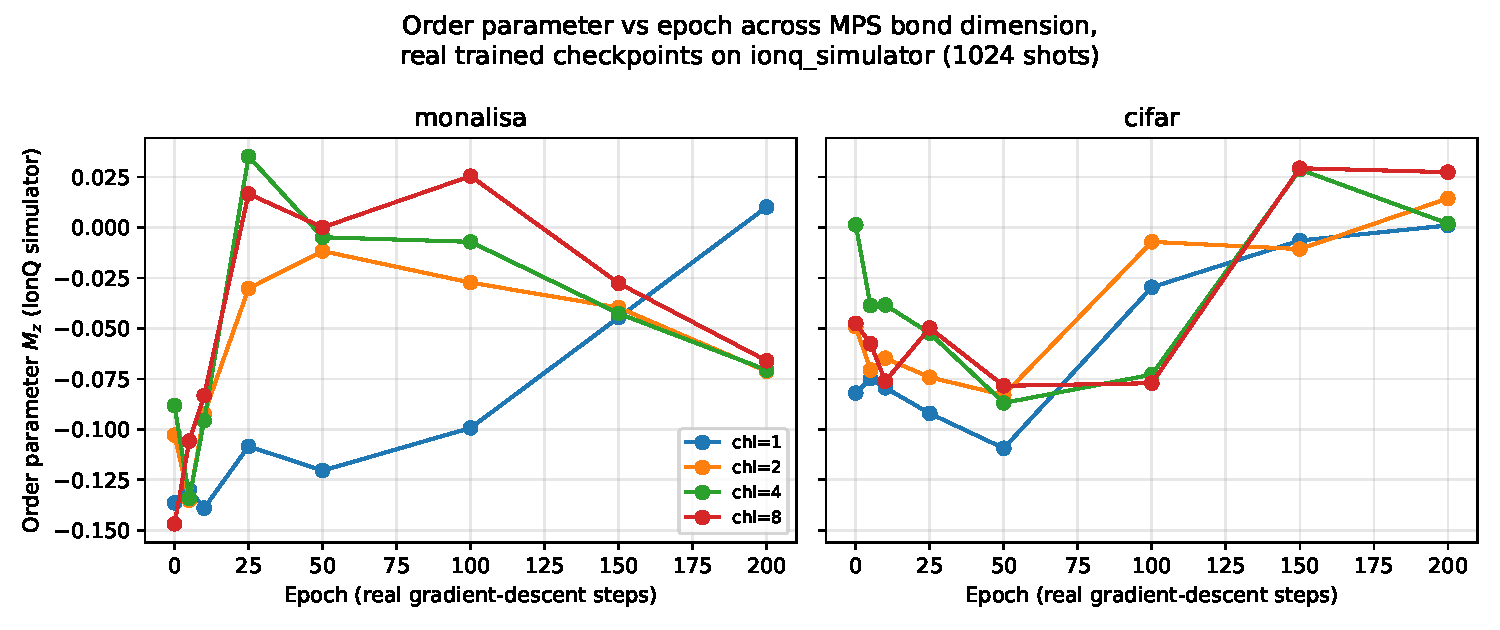
\includegraphics[width=0.9\linewidth]{figures/checkpoint_ionq_bond_dimension_order_parameter.pdf}
\caption{The same bond-dimension checkpoint replay as Figure~\ref{fig:supp_checkpoint_hardware_bond_dimension}, executed instead on the IonQ ideal cloud simulator at 1024 shots.}
\label{fig:supp_checkpoint_ionq_bond_dimension}
\end{figure}

Figure~\ref{fig:supp_checkpoint_ionq_bond_dimension} shows the corresponding IonQ traces: $\chi=1$ remains the most distinct trajectory on both images, the same qualitative pattern as Figure~\ref{fig:supp_checkpoint_hardware_bond_dimension}'s hardware replay, consistent with these being ideal-simulator and real-device executions of the identical checkpoint circuits rather than independent training runs.

We additionally replayed the three-basis energy-to-entanglement estimator for the same checkpoint grid. Each platform/shot job contains $2\times4\times8\times3=192$ circuits. At $\chi=1$, the MPS is a product state and the archived entropy sum is fixed at the numerical floor, $S=5.0\times10^{-6}$, compared with $S=0.014$--$0.045$ for $\chi\geq2$. Consequently, $R_{ES}=H/S$ reaches $O(10^5$--$10^6)$ through division by a near-zero denominator. We retain those rows in the machine-readable archive but exclude them from Figure~\ref{fig:supp_checkpoint_hardware_bond_dimension_res}; this is a construction-limit audit, not a physical divergence.

\begin{figure}[H]
\centering
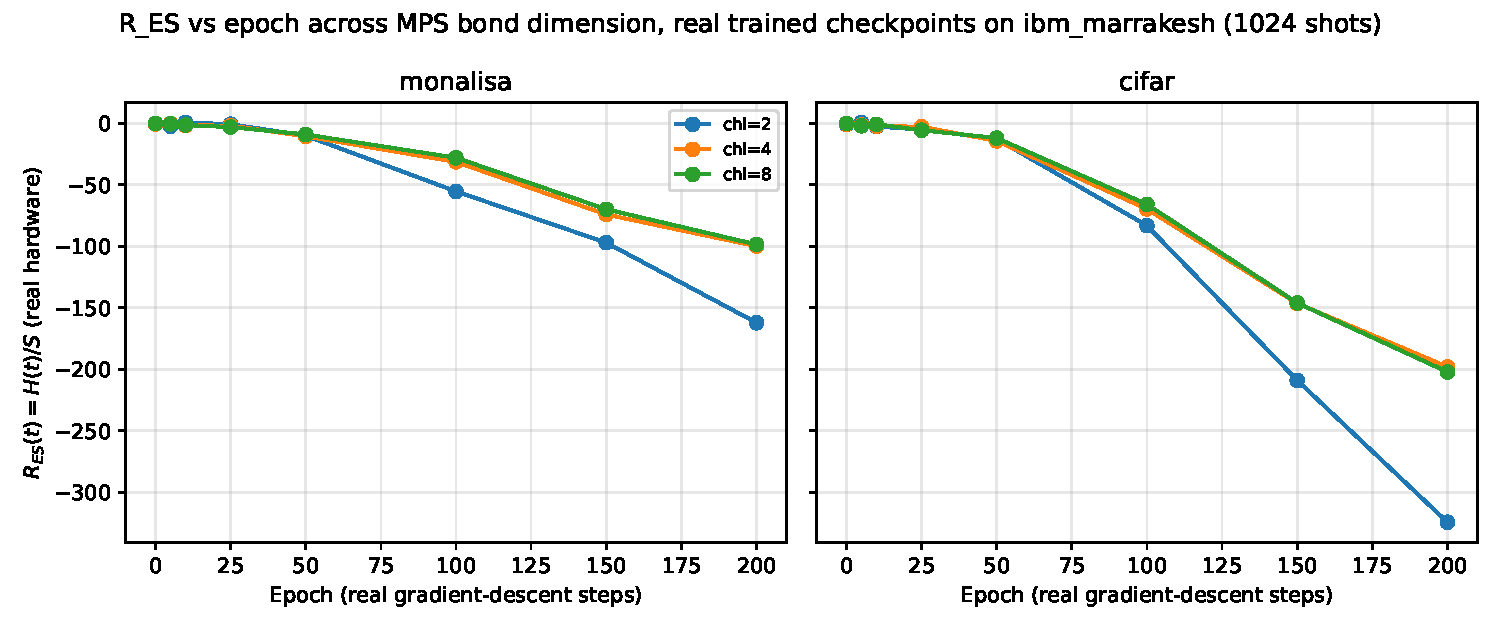
\includegraphics[width=0.9\linewidth]{figures/checkpoint_hardware_bond_dimension_r_es.pdf}
\caption{Energy-to-entanglement ratio across $\chi\in\{2,4,8\}$ at 1024 shots on real IBM Quantum hardware; $\chi=1$ is excluded because its product-state entropy is at the numerical floor.}
\label{fig:supp_checkpoint_hardware_bond_dimension_res}
\end{figure}

\begin{table}[H]
\centering
\caption{Bond-dimension $R_{ES}$ replay jobs. Each job contains 192 circuits over three measurement bases.}
\scriptsize
\resizebox{\linewidth}{!}{%
\begin{tabular}{llll}
\toprule
Platform & Backend & Shots & Job ID \\
\midrule
IBM hardware & \texttt{ibm\_marrakesh} & 256 & \texttt{d9hr44shonhs73adgq40} \\
IBM hardware & \texttt{ibm\_marrakesh} & 512 & \texttt{d9hr5u50k0jc738ilbs0} \\
IBM hardware & \texttt{ibm\_marrakesh} & 1024 & \texttt{d9hrb8shonhs73adh8mg} \\
IonQ ideal simulator & \texttt{ionq\_simulator} & 256 & \texttt{019f957f-dfbe-70fc-b6aa-b2398317f049} \\
IonQ ideal simulator & \texttt{ionq\_simulator} & 512 & \texttt{019f9584-4ba3-7224-ab7b-e81e32e6c1e2} \\
IonQ ideal simulator & \texttt{ionq\_simulator} & 1024 & \texttt{019f9586-4eb6-7596-ba47-dc6132c7f943} \\
\bottomrule
\end{tabular}
}
\end{table}

\begin{figure}[H]
\centering
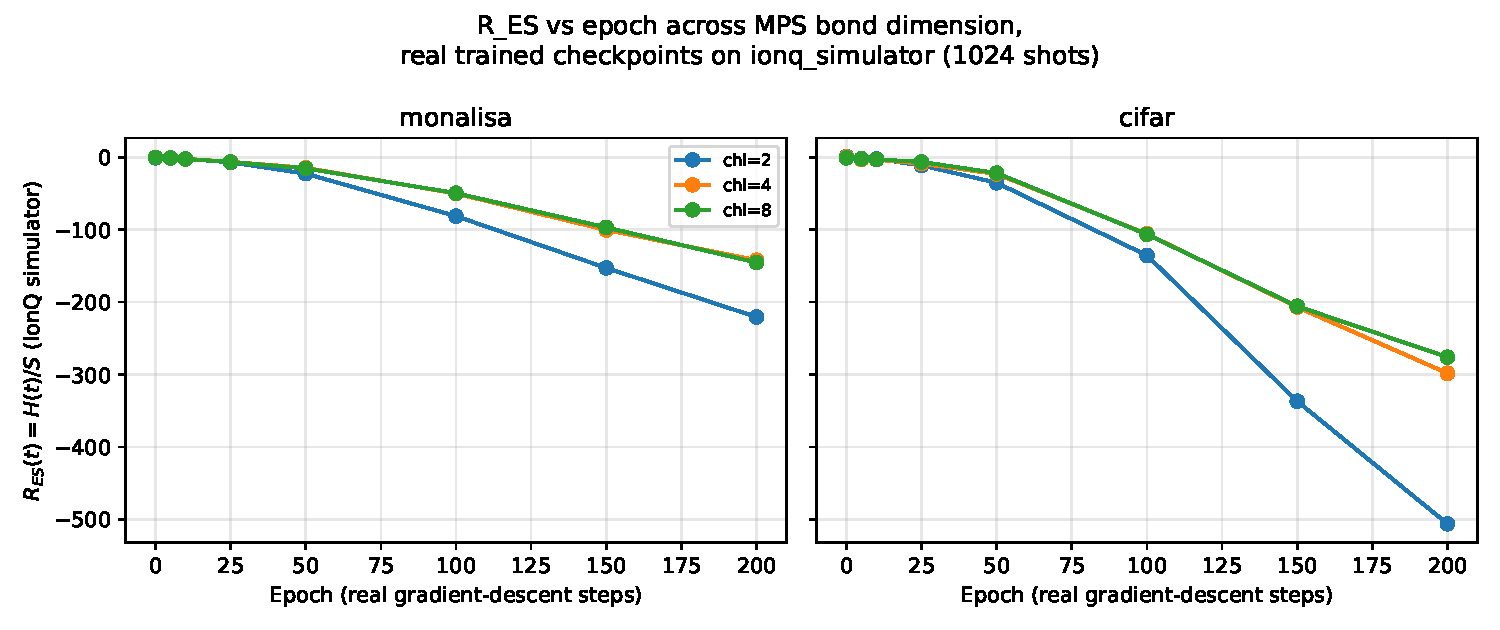
\includegraphics[width=0.9\linewidth]{figures/checkpoint_ionq_bond_dimension_r_es.pdf}
\caption{Energy-to-entanglement ratio across $\chi\in\{2,4,8\}$ at 1024 shots on the IonQ ideal cloud simulator, the same checkpoints and circuits as Figure~\ref{fig:supp_checkpoint_hardware_bond_dimension_res}; $\chi=1$ is excluded for the same numerical-floor reason.}
\label{fig:supp_checkpoint_ionq_bond_dimension_res}
\end{figure}

For $\chi\in\{2,4,8\}$, the $\chi=4$ and $\chi=8$ traces are close on both images, while $\chi=2$ becomes more negative by epoch 200, on both real hardware (Figure~\ref{fig:supp_checkpoint_hardware_bond_dimension_res}) and the IonQ ideal simulator (Figure~\ref{fig:supp_checkpoint_ionq_bond_dimension_res}). This single-patch, single-seed pattern is descriptive. It neither establishes a bond-dimension scaling law nor independently confirms the two-seed simulator observation about initialization sensitivity. The complete per-shot IBM and IonQ summaries are stored under \path{IBM_Cloud/outputs/checkpoint_bond_dimension_hardware_sweep/} and \path{IBM_Cloud/outputs/checkpoint_bond_dimension_temperature_hardware_sweep/}.

\subsection{Reconstruction Decode}
Hardware counts were converted to observable expectation values by the standard parity estimator, $\langle Z_i\rangle = \frac{1}{S}\sum_{\text{shots}} (-1)^{b_i}$ (identically for $X$, $Y$ after basis rotation), with pairwise correlators computed as the shot-weighted mean of $(-1)^{b_i+b_j}$ within the same measurement basis. The resulting observable vector, concatenated with the training-time positional encoding, was passed through the \emph{unmodified} trained decoder. No hardware-specific fine-tuning, error mitigation, or post-hoc calibration was applied.

\section{Reproducibility and Artifact Map}\leavevmode\par
The repository-level experiment drivers set Python, NumPy, and PyTorch random seeds explicitly. Unless a section states otherwise, multi-seed studies use seeds $\{0,1,2,3,4\}$; the reduced real-circuit topology confirmation and six-dataset reconstruction extension use $\{0,1,2\}$. Held-out samples are disjoint from their corresponding fitting samples, and each reported paired test preserves the pairing unit stated in its table or surrounding text (image within split, or seed after within-seed image aggregation). ``Mean $\pm$ std'' denotes the arithmetic mean and population-standard-deviation summary (NumPy \texttt{ddof=0}) over the unit named in the caption. Bootstrap intervals are percentile 95\% intervals; Wilcoxon values are two-sided signed-rank tests. No multiple-comparison correction is applied, so $p$-values should be interpreted as individual-comparison summaries rather than as a family-wise discovery analysis.

The current verification environment uses Python 3.11.9, PyTorch 2.6.0 with CUDA 12.4, PennyLane 0.42.3, Qiskit 2.5.0, NumPy 2.4.6, pandas 3.0.3, scikit-learn 1.9.0, quimb 1.11.2, cotengra 0.7.5, and autoray 0.6.12 on an NVIDIA GeForce GTX 1050. The package constraints are declared in \path{pyproject.toml}; because that file does not pin every dependency to an exact version, the versions above identify the environment used for this verification pass rather than claiming bitwise reproducibility across arbitrary future installations.

\begin{sloppypar}
The principal artifact map is as follows. The lowercase driver \path{main2/newHVK/run_newhvk_suite.py} generates the synthetic restricted-pair diagnostic under \path{main2/newHVK/results/full_ablation_suite/} and the held-out CIFAR-10 controls under \path{main2/newHVK/results/q1_validation/}; the six-dataset extension is generated by \path{main2/newHVK/run_multi_dataset_validation.py} and stored under \path{main2/newHVK/results/multi_dataset_validation/}. The newer experiment drivers use the repository's historically uppercase path: \path{Main2/newHVK/run_topology_comparison.py}, \path{Main2/newHVK/run_d4_symmetry_experiment.py}, and \path{Main2/newHVK/run_phase_transition_multi_dataset.py}, with outputs respectively under \path{Main2/newHVK/results/topology_comparison/}, \path{Main2/newHVK/results/d4_symmetry_experiment/}, and \path{Main2/newHVK/results/phase_transition_multi_dataset/}. The topology directory includes raw per-run JSON, summaries, paired statistics, and a surrogate manifest. Excluded legacy training-mode traces and any future deterministic evaluation-mode traces have distinct filenames and provenance fields. Path case is intentional and must be preserved on case-sensitive systems. Hardware-pilot result metadata and measured observable arrays are stored under \path{IBM_Cloud/outputs/hardware_reconstruction/} and \path{IBM_Cloud/outputs/hvk2d_cifar_hardware_reconstruction/}; bond-dimension hardware replays use the two output directories listed in Section~\ref{sec:supp_bond_dimension_hardware}. Raw and summary artifacts are retained separately so that manuscript means and uncertainty intervals can be recomputed without reading values from figures.
\end{sloppypar}

\section{Discussion}

\subsection{Task-Dependent Representational Scope}
The tie-with-classical outcome in Section~\ref{sec:holdout_headline} is consistent with a broader pattern in quantum machine learning: whether a quantum feature map or kernel offers an advantage over a classical model depends on the data, target, and comparison class rather than on the model label alone. At the resolution and patch size tested here, the empirical result is that local and raw-linear maps already capture the reconstruction signal available to the shared readout; we do not infer an entanglement property of the image distribution from that observation. The restricted diagnostic of Section~\ref{sec:restricted_ablation} is the contrasting case: its target is constructed around a distant-element product that the tested raw or local features cannot represent under the fixed linear readout, and the entangling channel separates in that setting. Together, the results delimit the tested operating regime: entangling observables are necessary within the restricted feature/readout class, but are not isolated as necessary for ordinary held-out reconstruction under the evaluated protocol.

\subsection{Design and Evaluation Guidelines}
We distill this ablation study into concrete guidance for evaluating hybrid quantum--classical vision models: (1) \emph{resource-match} every classical control to the quantum model's feature width and readout parameter count; (2) \emph{freeze-isolate} each trainable component independently before crediting any one of them with an observed gain; (3) \emph{audit every favorable diagnostic for target--feature leakage} by tracing target- and feature-construction code for shared subexpressions; (4) \emph{report held-out, not same-set, performance} as the primary evidence for a representation-learning claim; (5) \emph{report multiple seeds with error bars} on any comparison intended to support a quantitative claim.

\section{Conclusion}
The resource-matched, multi-seed study delineates the tested operating regime of HVK. Under a shared fitted readout, simple local/raw maps match or exceed the HVK2D pair-observable map on ordinary held-out reconstruction. The entangling observable channel separates on the restricted target constructed to require nonlocal correlations; separately, $D_4$ pooling enforces equivariance to numerical precision but does not improve held-out reconstruction accuracy in the tested experiment. On held-out CIFAR-10, local-observable and raw-linear controls reach $18.80\pm1.42$~dB compared with HVK2D's $18.12\pm1.54$~dB; seed-level inference gives a $-0.68$~dB HVK2D-minus-control difference (bootstrap 95\% CI $[-0.91,-0.46]$~dB; Wilcoxon $p=0.0625$, $n=5$). The same numerical direction appears on five further real datasets. These results motivate task-aligned HVK variants and strengthen the framework's evidentiary scope. The leakage and provenance audits contribute a transferable validation protocol, and Section~\ref{sec:hardware_methodology} provides the complete hardware-pilot methodology.

\begin{thebibliography}{9}
\bibitem{IonQBackends} IonQ, ``Backends,'' \textit{IonQ Quantum Cloud Documentation}. [Online]. Available: \url{https://docs.ionq.com/user-manual/backends}. Accessed: Jul. 24, 2026.
\bibitem{Schuirmann1987TOST} D. J. Schuirmann, ``A comparison of the two one-sided tests procedure and the power approach for assessing the equivalence of average bioavailability,'' \textit{Journal of Pharmacokinetics and Biopharmaceutics}, vol. 15, no. 6, pp. 657--680, 1987, doi: 10.1007/BF01068419.
\bibitem{Lakens2017TOST} D. Lakens, ``Equivalence tests: A practical primer for $t$ tests, correlations, and meta-analyses,'' \textit{Social Psychological and Personality Science}, vol. 8, no. 4, pp. 355--362, 2017, doi: 10.1177/1948550617697177.
\bibitem{Krizhevsky2009} A. Krizhevsky, ``Learning multiple layers of features from tiny images,'' University of Toronto, Technical Report, 2009.
\bibitem{LeCun1998} Y. LeCun, L. Bottou, Y. Bengio, and P. Haffner, ``Gradient-based learning applied to document recognition,'' \textit{Proceedings of the IEEE}, vol. 86, no. 11, pp. 2278--2324, 1998, doi: 10.1109/5.726791.
\bibitem{Xiao2017} H. Xiao, K. Rasul, and R. Vollgraf, ``Fashion-MNIST: A novel image dataset for benchmarking machine learning algorithms,'' arXiv:1708.07747, 2017.
\bibitem{Yang2023} J. Yang et al., ``MedMNIST v2---A large-scale lightweight benchmark for 2D and 3D biomedical image classification,'' \textit{Scientific Data}, vol. 10, Art. no. 41, 2023, doi: 10.1038/s41597-022-01721-8.
\bibitem{Wolberg1993} W. Wolberg, O. Mangasarian, N. Street, and W. Street, ``Breast Cancer Wisconsin (Diagnostic),'' UCI Machine Learning Repository, 1993, doi: 10.24432/C5DW2B.
\bibitem{Xu2021} R. Xu, X. Wang, K. Chen, B. Zhou, and C. C. Loy, ``Positional Encoding as Spatial Inductive Bias in GANs,'' in \textit{Proceedings of the IEEE/CVF Conference on Computer Vision and Pattern Recognition (CVPR)}, 2021, pp. 13564--13573.
\end{thebibliography}

\end{document}
